%&preformat-synopsis
\RequirePackage[l2tabu,orthodox]{nag} % Раскомментировав, можно в логе получать рекомендации относительно правильного использования пакетов и предупреждения об устаревших и нерекомендуемых пакетах

% Откомментируйте, чтобы отключить генерацию закладок в pdf
% \PassOptionsToPackage{bookmarks=false}{hyperref}
\documentclass[a5paper,10pt,twoside,openany,article]{memoir} %,draft
%\usepackage[english]{babel}

%%%%%%%%%%%%%%%%%%%%%%%%%%%%%%%%%%%%%%%%%%%%%%%%%%%%%%%%%%%%%%%%%%%%%%%%%%%%%%%%
%%%% Файл упрощённых настроек шаблона, общих для диссертации и автореферата %%%%
%%%%%%%%%%%%%%%%%%%%%%%%%%%%%%%%%%%%%%%%%%%%%%%%%%%%%%%%%%%%%%%%%%%%%%%%%%%%%%%%

%%% Режим черновика %%%
\makeatletter
\@ifundefined{c@draft}{
  \newcounter{draft}
  \setcounter{draft}{0}  % 0 --- чистовик (максимальное соблюдение ГОСТ)
                         % 1 --- черновик (отклонения от ГОСТ, но быстрая
                         %       сборка итоговых PDF)
}{}
\@ifundefined{myspec}{
  \newcounter{myspec}
  \setcounter{myspec}{1}  % 0 --- 05.13.18
                         % 1 --- 27.03.03
}{}
\makeatother

%%% Пометки в тексте %%%
\makeatletter
\@ifundefined{c@showmarkup}{
  \newcounter{showmarkup}
  \setcounter{showmarkup}{0}  % 0 --- скрыть пометки
                              % 1 --- показывать пометки
}{}
\makeatother

%%% Использование в pdflatex шрифтов не по-умолчанию %%%
\makeatletter
\@ifundefined{c@usealtfont}{
  \newcounter{usealtfont}
  \setcounter{usealtfont}{1}    % 0 --- шрифты на базе Computer Modern
                                % 1 --- использовать пакет pscyr, при его
                                %       наличии
                                % 2 --- использовать пакет XCharter, при наличии
                                %       подходящей версии
}{}
\makeatother

%%% Использование в xelatex и lualatex семейств шрифтов %%%
\makeatletter
\@ifundefined{c@fontfamily}{
  \newcounter{fontfamily}
  \setcounter{fontfamily}{1}  % 0 --- CMU семейство. Используется как fallback;
                              % 1 --- Шрифты от MS (Times New Roman и компания)
                              % 2 --- Семейство Liberation
}{}
\makeatother

%%% Библиография %%%
\makeatletter
\@ifundefined{c@bibliosel}{
  \newcounter{bibliosel}
  \setcounter{bibliosel}{1}   % 0 --- встроенная реализация с загрузкой файла
                              %       через движок bibtex8;
                              % 1 --- реализация пакетом biblatex через движок
                              %       biber
}{}
\makeatother

%%% Вывод типов ссылок в библиографии %%%
\makeatletter
\@ifundefined{c@mediadisplay}{
  \newcounter{mediadisplay}
  \setcounter{mediadisplay}{1}   % 0 --- не делать ничего; надписи [Текст] и
                                 %       [Эл. ресурс] будут выводиться только в ссылках с
                                 %       заполненным полем `media`;
                                 % 1 --- автоматически добавлять надпись [Текст] к ссылкам с
                                 %       незаполненным полем `media`; таким образом, у всех
                                 %       источников будет указан тип, что соответствует
                                 %       требованиям ГОСТ
                                 % 2 --- автоматически удалять надписи [Текст], [Эл. Ресурс] и др.;
                                 %       не соответствует ГОСТ
                                 % 3 --- автоматически удалять надпись [Текст];
                                 %       не соответствует ГОСТ
                                 % 4 --- автоматически удалять надпись [Эл. Ресурс];
                                 %       не соответствует ГОСТ
}{}
\makeatother

%%% Предкомпиляция tikz рисунков для ускорения работы %%%
\makeatletter
\@ifundefined{c@imgprecompile}{
  \newcounter{imgprecompile}
  \setcounter{imgprecompile}{0}   % 0 --- без предкомпиляции;
                                  % 1 --- пользоваться предварительно
                                  %       скомпилированными pdf вместо генерации
                                  %       заново из tikz
}{}
\makeatother
          % общие настройки шаблона

%%% Поля и разметка страницы %%%
\usepackage{pdflscape}  % Для включения альбомных страниц
\usepackage{geometry}   % Для последующего задания полей
\usepackage{listings}

%%% Проверка используемого TeX-движка %%%
\newif\ifxetexorluatex   % определяем новый условный оператор (http://tex.stackexchange.com/a/47579)
\ifxetex
    \xetexorluatextrue
\else
    \ifluatex
        \xetexorluatextrue
    \else
        \xetexorluatexfalse
    \fi
\fi

\newif\ifsynopsis           % Условие, проверяющее, что документ --- автореферат

\providebool{presentation}

\usepackage{comment}    % Позволяет убирать блоки текста (добавляет
                        % окружение comment и команду \excludecomment)

%%% Математические пакеты %%%
\usepackage{amsthm,amsmath,amscd}   % Математические дополнения от AMS
\usepackage{amsfonts,amssymb}       % Математические дополнения от AMS
\usepackage{mathtools}              % Добавляет окружение multlined
\usepackage{xfrac}                  % Красивые дроби
\usepackage[
    locale = DE,
    list-separator       = {;\,},
    list-final-separator = {;\,},
    list-pair-separator  = {;\,},
    list-units           = single,
    range-units          = single,
    range-phrase={\text{\ensuremath{-}}},
    % quotient-mode        = fraction, % красивые дроби могут не соответствовать ГОСТ
    fraction-function    = \sfrac,
    separate-uncertainty,
    ]{siunitx}[=v2]                 % Размерности SI
\sisetup{inter-unit-product = \ensuremath{{}\cdot{}}}

% Кириллица в нумерации subequations
% Для правильной работы требуется выполнение сразу после загрузки пакетов
\patchcmd{\subequations}{\def\theequation{\theparentequation\alph{equation}}}
{\def\theequation{\theparentequation\asbuk{equation}}}
{\typeout{subequations patched}}{\typeout{subequations not patched}}

%%%% Установки для размера шрифта 14 pt %%%%
%% Формирование переменных и констант для сравнения (один раз для всех подключаемых файлов)%%
%% должно располагаться до вызова пакета fontspec или polyglossia, потому что они сбивают его работу
\newlength{\curtextsize}
\newlength{\bigtextsize}
\setlength{\bigtextsize}{13.9pt}

\makeatletter
%\show\f@size    % неплохо для отслеживания, но вызывает стопорение процесса,
                 % если документ компилируется без команды  -interaction=nonstopmode
\setlength{\curtextsize}{\f@size pt}
\makeatother

%%% Кодировки и шрифты %%%
\ifxetexorluatex
    \ifpresentation
        \providecommand*\autodot{} % quick fix for polyglossia 1.50
    \fi
    \PassOptionsToPackage{no-math}{fontspec}    % https://tex.stackexchange.com/a/26295/104425
    \usepackage{polyglossia}[2014/05/21]        % Поддержка многоязычности
                                        % (fontspec подгружается автоматически)
\else
   %%% Решение проблемы копирования текста в буфер кракозябрами
    \ifnumequal{\value{usealtfont}}{0}{}{
        \input glyphtounicode.tex
        \input glyphtounicode-cmr.tex %from pdfx package
        \pdfgentounicode=1
    }
    \usepackage{cmap}   % Улучшенный поиск русских слов в полученном pdf-файле
    \ifnumequal{\value{usealtfont}}{2}{}{
        \defaulthyphenchar=127  % Если стоит до fontenc, то переносы
                                % не впишутся в выделяемый текст при
                                % копировании его в буфер обмена
    }
    \usepackage{textcomp}
    \usepackage[T1,T2A]{fontenc}                    % Поддержка русских букв
    \ifnumequal{\value{usealtfont}}{1}{% Используется pscyr, при наличии
        \IfFileExists{pscyr.sty}{\usepackage{pscyr}}{}  % Подключение pscyr
    }{}
    \usepackage[utf8]{inputenc}[2014/04/30]         % Кодировка utf8
    \usepackage[english, russian]{babel}[2014/03/24]% Языки: русский, английский
    \makeatletter\AtBeginDocument{\let\@elt\relax}\makeatother % babel 3.40 fix
    \ifnumequal{\value{usealtfont}}{2}{
        % http://dxdy.ru/post1238763.html#p1238763
        \usepackage[scaled=0.914]{XCharter}[2017/12/19] % Подключение русифицированных шрифтов XCharter
        \usepackage[charter, vvarbb, scaled=1.048]{newtxmath}[2017/12/14]
        \ifpresentation
        \else
            \setDisplayskipStretch{-0.078}
        \fi
    }{}
\fi

%%% Оформление абзацев %%%
\ifpresentation
\else
    \indentafterchapter     % Красная строка после заголовков типа chapter
    \usepackage{indentfirst}
\fi

%%% Цвета %%%
\ifpresentation
\else
    \usepackage[dvipsnames, table, hyperref]{xcolor} % Совместимо с tikz
\fi

%%% Таблицы %%%
\usepackage{longtable,ltcaption} % Длинные таблицы
\usepackage{multirow,makecell}   % Улучшенное форматирование таблиц
\usepackage{tabu, tabulary}      % таблицы с автоматически подбирающейся
                                 % шириной столбцов (tabu обязательно
                                 % до hyperref вызывать)
\makeatletter
%https://github.com/tabu-issues-for-future-maintainer/tabu/issues/26
\@ifpackagelater{longtable}{2020/02/07}{
\def\tabuendlongtrial{%
    \LT@echunk  \global\setbox\LT@gbox \hbox{\unhbox\LT@gbox}\kern\wd\LT@gbox
                \LT@get@widths
}%
}{}
\makeatother

\usepackage{threeparttable}      % автоматический подгон ширины подписи таблицы

%%% Общее форматирование
\usepackage{soulutf8}% Поддержка переносоустойчивых подчёркиваний и зачёркиваний
\usepackage{icomma}  % Запятая в десятичных дробях

%%% Оптимизация расстановки переносов и длины последней строки абзаца
\IfFileExists{impnattypo.sty}{% проверка установленности пакета impnattypo
    \ifluatex
        \ifnumequal{\value{draft}}{1}{% Черновик
            \usepackage[hyphenation, lastparline, nosingleletter, homeoarchy,
            rivers, draft]{impnattypo}
        }{% Чистовик
            \usepackage[hyphenation, lastparline, nosingleletter]{impnattypo}
        }
    \else
        \usepackage[hyphenation, lastparline]{impnattypo}
    \fi
}{}

%% Векторная графика

\usepackage{tikz}                   % Продвинутый пакет векторной графики
\usetikzlibrary{chains}             % Для примера tikz рисунка
\usetikzlibrary{shapes.geometric}   % Для примера tikz рисунка
\usetikzlibrary{shapes.symbols}     % Для примера tikz рисунка
\usetikzlibrary{arrows}             % Для примера tikz рисунка

%%% Гиперссылки %%%
\ifxetexorluatex
    \let\CYRDZE\relax
\fi
\usepackage{hyperref}[2012/11/06]

%%% Изображения %%%
\usepackage{graphicx}[2014/04/25]   % Подключаем пакет работы с графикой
\usepackage{caption}                % Подписи рисунков и таблиц
\usepackage{subcaption}             % Подписи подрисунков и подтаблиц
\usepackage{pdfpages}               % Добавление внешних pdf файлов

%%% Счётчики %%%
\usepackage{aliascnt}
\usepackage[figure,table]{totalcount}   % Счётчик рисунков и таблиц
\usepackage{totcount}   % Пакет создания счётчиков на основе последнего номера
                        % подсчитываемого элемента (может требовать дважды
                        % компилировать документ)
\usepackage{totpages}   % Счётчик страниц, совместимый с hyperref (ссылается
                        % на номер последней страницы). Желательно ставить
                        % последним пакетом в преамбуле

%%% Продвинутое управление групповыми ссылками (пока только формулами) %%%
\ifpresentation
\else
    \usepackage[russian]{cleveref} % cleveref имеет сложности со считыванием
    % языка из babel. Такое решение русификации вывода выбрано вместо
    % определения в documentclass из опасности что-то лишнее передать во все
    % остальные пакеты, включая библиографию.

    % Добавление возможности использования пробелов в \labelcref
    % https://tex.stackexchange.com/a/340502/104425
    \usepackage{kvsetkeys}
    \makeatletter
    \let\org@@cref\@cref
    \renewcommand*{\@cref}[2]{%
        \edef\process@me{%
            \noexpand\org@@cref{#1}{\zap@space#2 \@empty}%
        }\process@me
    }
    \makeatother
\fi

\usepackage{placeins} % для \FloatBarrier

\ifnumequal{\value{draft}}{1}{% Черновик
    \usepackage[firstpage]{draftwatermark}
    \SetWatermarkText{DRAFT}
    \SetWatermarkFontSize{14pt}
    \SetWatermarkScale{15}
    \SetWatermarkAngle{45}
}{}

%%% Цитата, не приводимая в автореферате:
% возможно, актуальна только для biblatex
%\newcommand{\citeinsynopsis}[1]{\ifsynopsis\else ~\cite{#1} \fi}

% если текущий процесс запущен библиотекой tikz-external, то прекомпиляция должна быть включена
\ifdefined\tikzexternalrealjob
    \setcounter{imgprecompile}{1}
\fi

\ifnumequal{\value{imgprecompile}}{1}{% Только если у нас включена предкомпиляция
    \usetikzlibrary{external}   % подключение возможности предкомпиляции
    \tikzexternalize[prefix=images/cache/,optimize command away=\includepdf] % activate! % здесь можно указать отдельную папку для скомпилированных файлов
    \ifxetex
        \tikzset{external/up to date check={diff}}
    \fi
}{}
       % Пакеты общие для диссертации и автореферата
\synopsistrue                 % Этот документ --- автореферат
%%% Опционально %%%
% Следующий пакет может быть полезен, если надо ужать текст, чтобы сам текст не править, но чтобы места он занимал поменьше
%\usepackage{savetrees}

%%% Списки %%%
\usepackage{enumitem}
\usepackage{titlesec}

% Этот пакет может быть полезен для печати текста брошюрой
%\usepackage[print]{booklet}
  % Пакеты для автореферата
%%% Микротипографика %%%
%\ifnumequal{\value{draft}}{0}{% Только если у нас режим чистовика
%    \usepackage[final]{microtype}[2016/05/14] % улучшает представление букв и слов в строках, может помочь при наличии отдельно висящих слов
%}{}
 % Пакеты для специфических пользовательских задач

% Новые переменные, которые могут использоваться во всём проекте
% ГОСТ 7.0.11-2011
% 9.2 Оформление текста автореферата диссертации
% 9.2.1 Общая характеристика работы включает в себя следующие основные структурные
% элементы:
% актуальность темы исследования;
\newcommand{\actualityTXT}{Актуальность темы.}
% степень ее разработанности;
\newcommand{\progressTXT}{Степень разработанности темы.}
% цели и задачи;
\newcommand{\aimTXT}{Целью}
\newcommand{\tasksTXT}{задачи}
% научную новизну;
\newcommand{\noveltyTXT}{Научная новизна:}
% теоретическую и практическую значимость работы;
%\newcommand{\influenceTXT}{Теоретическая и практическая значимость}
% или чаще используют просто
\newcommand{\influenceTXT}{Практическая значимость}
% методологию и методы исследования;
\newcommand{\methodsTXT}{Методология и методы исследования.}
% положения, выносимые на защиту;
\newcommand{\defpositionsTXT}{Основные положения, выносимые на~защиту:}
% степень достоверности и апробацию результатов.
\newcommand{\reliabilityTXT}{Достоверность}
\newcommand{\probationTXT}{Апробация работы.}

\newcommand{\contributionTXT}{Личный вклад.}
\newcommand{\publicationsTXT}{Публикации.}


%%% Заголовки библиографии:

% для автореферата:
\newcommand{\bibtitleauthor}{Публикации автора по теме диссертации}

% для стиля библиографии `\insertbiblioauthorgrouped`
\newcommand{\bibtitleauthorvak}{В изданиях из списка ВАК РФ}
\newcommand{\bibtitleauthorscopus}{В изданиях, входящих в международную базу цитирования Scopus}
\newcommand{\bibtitleauthorwos}{В изданиях, входящих в международную базу цитирования Web of Science}
\newcommand{\bibtitleauthorother}{В прочих изданиях}
\newcommand{\bibtitleauthorconf}{В сборниках трудов конференций}
\newcommand{\bibtitleauthorpatent}{Зарегистрированные патенты}
\newcommand{\bibtitleauthorprogram}{Зарегистрированные программы для ЭВМ}

% для стиля библиографии `\insertbiblioauthorimportant`:
\newcommand{\bibtitleauthorimportant}{Наиболее значимые \protect\MakeLowercase\bibtitleauthor}

% для списка литературы в диссертации и списка чужих работ в автореферате:
\newcommand{\bibtitlefull}{Список литературы} % (ГОСТ Р 7.0.11-2011, 4)
       % Новые переменные, которые могут использоваться во всём проекте
%%%%%%%%%%%%%%%%%%%%%%%%%%%%%%%%%%%%%%%%%%%%%%%%%%%%%%%
%%%% Файл упрощённых настроек шаблона автореферата %%%%
%%%%%%%%%%%%%%%%%%%%%%%%%%%%%%%%%%%%%%%%%%%%%%%%%%%%%%%

%%% Инициализирование переменных, не трогать!  %%%
\newcounter{showperssign}
\newcounter{showsecrsign}
\newcounter{showopplead}
%%%%%%%%%%%%%%%%%%%%%%%%%%%%%%%%%%%%%%%%%%%%%%%%%%%%%%%

\newcommand{\mycite}[2]{~[#2]}

%%% Список публикаций %%%
\makeatletter
\@ifundefined{c@usefootcite}{
  \newcounter{usefootcite}
  \setcounter{usefootcite}{1} % 0 --- два списка литературы;
                              % 1 --- список публикаций автора + цитирование
                              %       других работ в сносках
}{}
\makeatother

\makeatletter
\@ifundefined{c@bibgrouped}{
  \newcounter{bibgrouped}
  \setcounter{bibgrouped}{0}  % 0 --- единый список работ автора;
                              % 1 --- сгруппированные работы автора
}{}
\makeatother

%%% Область упрощённого управления оформлением %%%

%% Управление зазором между подрисуночной подписью и основным текстом %%
\setlength{\belowcaptionskip}{10pt plus 20pt minus 2pt}


%% Подпись таблиц %%

% смещение строк подписи после первой
\newcommand{\tabindent}{0cm}

% тип форматирования таблицы
% plain --- название и текст в одной строке
% split --- название и текст в разных строках
\newcommand{\tabformat}{plain}

%%% настройки форматирования таблицы `plain'

% выравнивание по центру подписи, состоящей из одной строки
% true  --- выравнивать
% false --- не выравнивать
\newcommand{\tabsinglecenter}{false}

% выравнивание подписи таблиц
% justified   --- выравнивать как обычный текст
% centering   --- выравнивать по центру
% centerlast  --- выравнивать по центру только последнюю строку
% centerfirst --- выравнивать по центру только первую строку
% raggedleft  --- выравнивать по правому краю
% raggedright --- выравнивать по левому краю
\newcommand{\tabjust}{justified}

% Разделитель записи «Таблица #» и названия таблицы
\newcommand{\tablabelsep}{~\cyrdash\ }

%%% настройки форматирования таблицы `split'

% положение названия таблицы
% \centering   --- выравнивать по центру
% \raggedleft  --- выравнивать по правому краю
% \raggedright --- выравнивать по левому краю
\newcommand{\splitformatlabel}{\raggedleft}

% положение текста подписи
% \centering   --- выравнивать по центру
% \raggedleft  --- выравнивать по правому краю
% \raggedright --- выравнивать по левому краю
\newcommand{\splitformattext}{\raggedright}

%% Подпись рисунков %%
%Разделитель записи «Рисунок #» и названия рисунка
\newcommand{\figlabelsep}{~\cyrdash\ }  % (ГОСТ 2.105, 4.3.1)
                                        % "--- здесь не работает

%Демонстрация подписи диссертанта на автореферате
\setcounter{showperssign}{1}  % 0 --- не показывать;
                              % 1 --- показывать
%Демонстрация подписи учёного секретаря на автореферате
\setcounter{showsecrsign}{1}  % 0 --- не показывать;
                              % 1 --- показывать
%Демонстрация информации об оппонентах и ведущей организации на автореферате
\setcounter{showopplead}{1}   % 0 --- не показывать;
                              % 1 --- показывать

%%% Цвета гиперссылок %%%
% Latex color definitions: http://latexcolor.com/
\definecolor{linkcolor}{rgb}{0.9,0,0}
\definecolor{citecolor}{rgb}{0,0.6,0}
\definecolor{urlcolor}{rgb}{0,0,1}
%\definecolor{linkcolor}{rgb}{0,0,0} %black
%\definecolor{citecolor}{rgb}{0,0,0} %black
%\definecolor{urlcolor}{rgb}{0,0,0} %black
        % Упрощённые настройки шаблона

%%% Основные сведения %%%
\newcommand{\thesisAuthorLastName}{Тюнин}
\newcommand{\thesisAuthorOtherNames}{Николай Николаевич}
\newcommand{\thesisAuthorInitials}{Н.\,Н.}
\newcommand{\thesisAuthor}             % Диссертация, ФИО автора
{%
    \texorpdfstring{% \texorpdfstring takes two arguments and uses the first for (La)TeX and the second for pdf
        \thesisAuthorLastName~\thesisAuthorOtherNames% так будет отображаться на титульном листе или в тексте, где будет использоваться переменная
    }{%
        \thesisAuthorLastName, \thesisAuthorOtherNames% эта запись для свойств pdf-файла. В таком виде, если pdf будет обработан программами для сбора библиографических сведений, будет правильно представлена фамилия.
    }
}
\newcommand{\thesisAuthorShort}        % Диссертация, ФИО автора инициалами
{\thesisAuthorInitials~\thesisAuthorLastName}
%\newcommand{\thesisUdk}                % Диссертация, УДК
%{\fixme{xxx.xxx}}
\newcommand{\thesisTitle}              % Диссертация, название
{Анализ и решение задач оптимизации направленности фазированных антенных решеток коротковолнового диапазона}

\ifnumequal{\value{myspec}}{0}{
    \newcommand{\thesisSpecialtyNumber}    % Диссертация, специальность, номер
    {05.13.18}
    \newcommand{\thesisSpecialtyTitle}     % Диссертация, специальность, название (название взято с сайта ВАК для примера)
    {Математическое моделирование, численные методы и~комплексы программ}
}{
    \newcommand{\thesisSpecialtyNumber}    % Диссертация, специальность, номер
    {2.3.1}
    \newcommand{\thesisSpecialtyTitle}     % Диссертация, специальность, название (название взято с сайта ВАК для примера)
    {Системный анализ, управление и обработка информации}
}

%% \newcommand{\thesisSpecialtyTwoNumber} % Диссертация, вторая специальность, номер
%% {\fixme{XX.XX.XX}}
%% \newcommand{\thesisSpecialtyTwoTitle}  % Диссертация, вторая специальность, название
%% {\fixme{Теория и~методика физического воспитания, спортивной тренировки,
%% оздоровительной и~адаптивной физической культуры}}
\newcommand{\thesisDegree}             % Диссертация, ученая степень
{кандидата технических наук}
\newcommand{\thesisDegreeShort}        % Диссертация, ученая степень, краткая запись
{канд. тех. наук}
\newcommand{\thesisCity}               % Диссертация, город написания диссертации
{Омск}
\newcommand{\thesisYear}               % Диссертация, год написания диссертации
{\the\year}
\newcommand{\thesisOrganization}       % Диссертация, организация
{Омский филиал Федерального государственного бюджетного учреждения науки Института математики им. С.Л. Соболева Сибирского отделения Российской академии наук (ОФ ИМ СО РАН)}
\newcommand{\thesisOrganizationShort}  % Диссертация, краткое название организации для доклада
{Оптимизация направленности}

\newcommand{\thesisInOrganization}     % Диссертация, организация в предложном падеже: Работа выполнена в ...
{Омском филиале Федерального государственного бюджетного учреждения науки Института математики им. С.Л. Соболева Сибирского отделения Российской академии наук (ОФ ИМ СО РАН)}

%% \newcommand{\supervisorDead}{}           % Рисовать рамку вокруг фамилии
\newcommand{\supervisorFio}              % Научный руководитель, ФИО
{Еремеев Антон Валентинович}
\newcommand{\supervisorRegalia}          % Научный руководитель, регалии
{доктор~физико-математических~наук,~доцент}
\newcommand{\supervisorFioShort}         % Научный руководитель, ФИО
{А.\,В.~Евемеев}
\newcommand{\supervisorRegaliaShort}     % Научный руководитель, регалии
{д.ф.-м.н.,~доц.}

%% \newcommand{\supervisorTwoDead}{}        % Рисовать рамку вокруг фамилии
%% \newcommand{\supervisorTwoFio}           % Второй научный руководитель, ФИО
%% {\fixme{Фамилия Имя Отчество}}
%% \newcommand{\supervisorTwoRegalia}       % Второй научный руководитель, регалии
%% {\fixme{уч. степень, уч. звание}}
%% \newcommand{\supervisorTwoFioShort}      % Второй научный руководитель, ФИО
%% {\fixme{И.\,О.~Фамилия}}
%% \newcommand{\supervisorTwoRegaliaShort}  % Второй научный руководитель, регалии
%% {\fixme{уч.~ст.,~уч.~зв.}}

\newcommand{\opponentOneFio}           % Оппонент 1, ФИО
{Картак Вадим Михайлович}
\newcommand{\opponentOneRegalia}       % Оппонент 1, регалии
{доктор физико-математических наук, профессор}
\newcommand{\opponentOneJobPlace}      % Оппонент 1, место работы
{Уфимский государственный авиационный технический университет}
\newcommand{\opponentOneJobPost}       % Оппонент 1, должность
{заведующий кафедрой}

\newcommand{\opponentTwoFio}           % Оппонент 2, ФИО
{Груздева Татьяна Владимировна}
\newcommand{\opponentTwoRegalia}       % Оппонент 2, регалии
{кандидат физико-математических наук}
\newcommand{\opponentTwoJobPlace}      % Оппонент 2, место работы
{Институт динамики систем и теории управления имени В.М. Матросова Сибирского отделения Российской академии наук}
\newcommand{\opponentTwoJobPost}       % Оппонент 2, должность
{старший научный сотрудник}

%% \newcommand{\opponentThreeFio}         % Оппонент 3, ФИО
%% {\fixme{Фамилия Имя Отчество}}
%% \newcommand{\opponentThreeRegalia}     % Оппонент 3, регалии
%% {\fixme{кандидат физико-математических наук}}
%% \newcommand{\opponentThreeJobPlace}    % Оппонент 3, место работы
%% {\fixme{Основное место работы c длинным длинным длинным длинным названием}}
%% \newcommand{\opponentThreeJobPost}     % Оппонент 3, должность
%% {\fixme{старший научный сотрудник}}

\newcommand{\leadingOrganizationTitle} % Ведущая организация, дополнительные строки. Удалить, чтобы не отображать в автореферате
{Федеральное государственное автономное образовательное учреждение высшего образования <<Омский государственный технический университет>>}

\newcommand{\defenseDate}              % Защита, дата
{"\underline{\phantom{0111}}"~~"\underline{\phantom{сентябрясент}}~\the\year~г.~в~\underline{\phantom{0111}}~часов}
\newcommand{\defenseCouncilNumber}     % Защита, номер диссертационного совета
{Д\,24.2.403.01}
\newcommand{\defenseCouncilTitle}      % Защита, учреждение диссертационного совета
{Сибирский государственный университет науки и технологий имени академика М.Ф. Решетнева}
\newcommand{\defenseCouncilAddress}    % Защита, адрес учреждение диссертационного совета
{660037 г. Красноярск, проспект имени газеты «Красноярский рабочий», 31}
\newcommand{\defenseCouncilPhone}      % Телефон для справок
{\fixme{+7~(0000)~00-00-00}}

\newcommand{\defenseSecretaryFio}      % Секретарь диссертационного совета, ФИО
{Панфилов Илья Александрович}
\newcommand{\defenseSecretaryRegalia}  % Секретарь диссертационного совета, регалии
{кандидат технических наук, доцент}            % Для сокращений есть ГОСТы, например: ГОСТ Р 7.0.12-2011 + http://base.garant.ru/179724/#block_30000

\newcommand{\synopsisLibrary}          % Автореферат, название библиотеки
{ФГБОУ ВО <<Сибирский государственный университет науки и технологий имени академика М.Ф. Решетнева>> и на сайте https://www.sibsau.ru}
\newcommand{\synopsisDate}             % Автореферат, дата рассылки
{"\underline{\phantom{0111}}"~~"\underline{\phantom{сентябрясент}}"~\the\year~года}

% To avoid conflict with beamer class use \providecommand
\providecommand{\keywords}%            % Ключевые слова для метаданных PDF диссертации и автореферата
{}
           % Основные сведения
%%% Кодировки и шрифты %%%
\ifxetexorluatex
    % Язык по-умолчанию русский с поддержкой приятных команд пакета babel
    \setmainlanguage[babelshorthands=true]{russian}
    % Дополнительный язык = английский (в американской вариации по-умолчанию)
    \setotherlanguage{english}

    % Проверка существования шрифтов. Недоступна в pdflatex
    \ifnumequal{\value{fontfamily}}{1}{
        \IfFontExistsTF{Times New Roman}{}{\setcounter{fontfamily}{0}}
    }{}
    \ifnumequal{\value{fontfamily}}{2}{
        \IfFontExistsTF{LiberationSerif}{}{\setcounter{fontfamily}{0}}
    }{}

    \ifnumequal{\value{fontfamily}}{0}{                    % Семейство шрифтов CMU. Используется как fallback
        \setmonofont{CMU Typewriter Text}                  % моноширинный шрифт
        \newfontfamily\cyrillicfonttt{CMU Typewriter Text} % моноширинный шрифт для кириллицы
        \defaultfontfeatures{Ligatures=TeX}                % стандартные лигатуры TeX, замены нескольких дефисов на тире и т. п. Настройки моноширинного шрифта должны идти до этой строки, чтобы при врезках кода программ в коде не применялись лигатуры и замены дефисов
        \setmainfont{CMU Serif}                            % Шрифт с засечками
        \newfontfamily\cyrillicfont{CMU Serif}             % Шрифт с засечками для кириллицы
        \setsansfont{CMU Sans Serif}                       % Шрифт без засечек
        \newfontfamily\cyrillicfontsf{CMU Sans Serif}      % Шрифт без засечек для кириллицы
    }

    \ifnumequal{\value{fontfamily}}{1}{                    % Семейство MS шрифтов
        \setmonofont{Courier New}                          % моноширинный шрифт
        \newfontfamily\cyrillicfonttt{Courier New}         % моноширинный шрифт для кириллицы
        \defaultfontfeatures{Ligatures=TeX}                % стандартные лигатуры TeX, замены нескольких дефисов на тире и т. п. Настройки моноширинного шрифта должны идти до этой строки, чтобы при врезках кода программ в коде не применялись лигатуры и замены дефисов
        \setmainfont{Times New Roman}                      % Шрифт с засечками
        \newfontfamily\cyrillicfont{Times New Roman}       % Шрифт с засечками для кириллицы
        \setsansfont{Arial}                                % Шрифт без засечек
        \newfontfamily\cyrillicfontsf{Arial}               % Шрифт без засечек для кириллицы
    }

    \ifnumequal{\value{fontfamily}}{2}{                    % Семейство шрифтов Liberation (https://pagure.io/liberation-fonts)
        \setmonofont{LiberationMono}[Scale=0.87] % моноширинный шрифт
        \newfontfamily\cyrillicfonttt{LiberationMono}[     % моноширинный шрифт для кириллицы
            Scale=0.87]
        \defaultfontfeatures{Ligatures=TeX}                % стандартные лигатуры TeX, замены нескольких дефисов на тире и т. п. Настройки моноширинного шрифта должны идти до этой строки, чтобы при врезках кода программ в коде не применялись лигатуры и замены дефисов
        \setmainfont{LiberationSerif}                      % Шрифт с засечками
        \newfontfamily\cyrillicfont{LiberationSerif}       % Шрифт с засечками для кириллицы
        \setsansfont{LiberationSans}                       % Шрифт без засечек
        \newfontfamily\cyrillicfontsf{LiberationSans}      % Шрифт без засечек для кириллицы
    }

\else
    \ifnumequal{\value{usealtfont}}{1}{% Используется pscyr, при наличии
        \IfFileExists{pscyr.sty}{\renewcommand{\rmdefault}{ftm}}{}
    }{}
\fi
          % Определение шрифтов (частичное)
%%% Шаблон %%%
\DeclareRobustCommand{\fixme}{\textcolor{red}}  % решаем проблему превращения
                                % названия цвета в результате \MakeUppercase,
                                % http://tex.stackexchange.com/a/187930,
                                % \DeclareRobustCommand protects \fixme
                                % from expanding inside \MakeUppercase
\AtBeginDocument{%
    \setlength{\parindent}{2.5em}                   % Абзацный отступ. Должен быть одинаковым по всему тексту и равен пяти знакам (ГОСТ Р 7.0.11-2011, 5.3.7).
}

%%% Таблицы %%%
\DeclareCaptionLabelSeparator{tabsep}{\tablabelsep} % нумерация таблиц
\DeclareCaptionFormat{split}{\splitformatlabel#1\par\splitformattext#3}

\captionsetup[table]{
        format=\tabformat,                % формат подписи (plain|hang)
        font=normal,                      % нормальные размер, цвет, стиль шрифта
        skip=.0pt,                        % отбивка под подписью
        parskip=.0pt,                     % отбивка между параграфами подписи
        position=above,                   % положение подписи
        justification=\tabjust,           % центровка
        indent=\tabindent,                % смещение строк после первой
        labelsep=tabsep,                  % разделитель
        singlelinecheck=\tabsinglecenter, % не выравнивать по центру, если умещается в одну строку
}

%%% Рисунки %%%
\DeclareCaptionLabelSeparator{figsep}{\figlabelsep} % нумерация рисунков

\captionsetup[figure]{
        format=plain,                     % формат подписи (plain|hang)
        font=normal,                      % нормальные размер, цвет, стиль шрифта
        skip=.0pt,                        % отбивка под подписью
        parskip=.0pt,                     % отбивка между параграфами подписи
        position=below,                   % положение подписи
        singlelinecheck=true,             % выравнивание по центру, если умещается в одну строку
        justification=centerlast,         % центровка
        labelsep=figsep,                  % разделитель
}

%%% Подписи подрисунков %%%
\DeclareCaptionSubType{figure}
\renewcommand\thesubfigure{\asbuk{subfigure}} % нумерация подрисунков
\ifsynopsis
\DeclareCaptionFont{norm}{\fontsize{10pt}{11pt}\selectfont}
\newcommand{\subfigureskip}{2.pt}
\else
\DeclareCaptionFont{norm}{\fontsize{14pt}{16pt}\selectfont}
\newcommand{\subfigureskip}{0.pt}
\fi

\captionsetup[subfloat]{
        labelfont=norm,                 % нормальный размер подписей подрисунков
        textfont=norm,                  % нормальный размер подписей подрисунков
        labelsep=space,                 % разделитель
        labelformat=brace,              % одна скобка справа от номера
        justification=centering,        % центровка
        singlelinecheck=true,           % выравнивание по центру, если умещается в одну строку
        skip=\subfigureskip,            % отбивка над подписью
        parskip=.0pt,                   % отбивка между параграфами подписи
        position=below,                 % положение подписи
}

%%% Настройки ссылок на рисунки, таблицы и др. %%%
% команды \cref...format отвечают за форматирование при помощи команды \cref
% команды \labelcref...format отвечают за форматирование при помощи команды \labelcref

\ifpresentation
\else
    \crefdefaultlabelformat{#2#1#3}

    % Уравнение
    \crefformat{equation}{(#2#1#3)} % одиночная ссылка с приставкой
    \labelcrefformat{equation}{(#2#1#3)} % одиночная ссылка без приставки
    \crefrangeformat{equation}{(#3#1#4) \cyrdash~(#5#2#6)} % диапазон ссылок с приставкой
    \labelcrefrangeformat{equation}{(#3#1#4) \cyrdash~(#5#2#6)} % диапазон ссылок без приставки
    \crefmultiformat{equation}{(#2#1#3)}{ и~(#2#1#3)}{, (#2#1#3)}{ и~(#2#1#3)} % перечисление ссылок с приставкой
    \labelcrefmultiformat{equation}{(#2#1#3)}{ и~(#2#1#3)}{, (#2#1#3)}{ и~(#2#1#3)} % перечисление без приставки

    % Подуравнение
    \crefformat{subequation}{(#2#1#3)} % одиночная ссылка с приставкой
    \labelcrefformat{subequation}{(#2#1#3)} % одиночная ссылка без приставки
    \crefrangeformat{subequation}{(#3#1#4) \cyrdash~(#5#2#6)} % диапазон ссылок с приставкой
    \labelcrefrangeformat{subequation}{(#3#1#4) \cyrdash~(#5#2#6)} % диапазон ссылок без приставки
    \crefmultiformat{subequation}{(#2#1#3)}{ и~(#2#1#3)}{, (#2#1#3)}{ и~(#2#1#3)} % перечисление ссылок с приставкой
    \labelcrefmultiformat{subequation}{(#2#1#3)}{ и~(#2#1#3)}{, (#2#1#3)}{ и~(#2#1#3)} % перечисление без приставки

    % Глава
    \crefformat{chapter}{#2#1#3} % одиночная ссылка с приставкой
    \labelcrefformat{chapter}{#2#1#3} % одиночная ссылка без приставки
    \crefrangeformat{chapter}{#3#1#4 \cyrdash~#5#2#6} % диапазон ссылок с приставкой
    \labelcrefrangeformat{chapter}{#3#1#4 \cyrdash~#5#2#6} % диапазон ссылок без приставки
    \crefmultiformat{chapter}{#2#1#3}{ и~#2#1#3}{, #2#1#3}{ и~#2#1#3} % перечисление ссылок с приставкой
    \labelcrefmultiformat{chapter}{#2#1#3}{ и~#2#1#3}{, #2#1#3}{ и~#2#1#3} % перечисление без приставки

    % Параграф
    \crefformat{section}{#2#1#3} % одиночная ссылка с приставкой
    \labelcrefformat{section}{#2#1#3} % одиночная ссылка без приставки
    \crefrangeformat{section}{#3#1#4 \cyrdash~#5#2#6} % диапазон ссылок с приставкой
    \labelcrefrangeformat{section}{#3#1#4 \cyrdash~#5#2#6} % диапазон ссылок без приставки
    \crefmultiformat{section}{#2#1#3}{ и~#2#1#3}{, #2#1#3}{ и~#2#1#3} % перечисление ссылок с приставкой
    \labelcrefmultiformat{section}{#2#1#3}{ и~#2#1#3}{, #2#1#3}{ и~#2#1#3} % перечисление без приставки

    % Приложение
    \crefformat{appendix}{#2#1#3} % одиночная ссылка с приставкой
    \labelcrefformat{appendix}{#2#1#3} % одиночная ссылка без приставки
    \crefrangeformat{appendix}{#3#1#4 \cyrdash~#5#2#6} % диапазон ссылок с приставкой
    \labelcrefrangeformat{appendix}{#3#1#4 \cyrdash~#5#2#6} % диапазон ссылок без приставки
    \crefmultiformat{appendix}{#2#1#3}{ и~#2#1#3}{, #2#1#3}{ и~#2#1#3} % перечисление ссылок с приставкой
    \labelcrefmultiformat{appendix}{#2#1#3}{ и~#2#1#3}{, #2#1#3}{ и~#2#1#3} % перечисление без приставки

    % Рисунок
    \crefformat{figure}{#2#1#3} % одиночная ссылка с приставкой
    \labelcrefformat{figure}{#2#1#3} % одиночная ссылка без приставки
    \crefrangeformat{figure}{#3#1#4 \cyrdash~#5#2#6} % диапазон ссылок с приставкой
    \labelcrefrangeformat{figure}{#3#1#4 \cyrdash~#5#2#6} % диапазон ссылок без приставки
    \crefmultiformat{figure}{#2#1#3}{ и~#2#1#3}{, #2#1#3}{ и~#2#1#3} % перечисление ссылок с приставкой
    \labelcrefmultiformat{figure}{#2#1#3}{ и~#2#1#3}{, #2#1#3}{ и~#2#1#3} % перечисление без приставки

    % Таблица
    \crefformat{table}{#2#1#3} % одиночная ссылка с приставкой
    \labelcrefformat{table}{#2#1#3} % одиночная ссылка без приставки
    \crefrangeformat{table}{#3#1#4 \cyrdash~#5#2#6} % диапазон ссылок с приставкой
    \labelcrefrangeformat{table}{#3#1#4 \cyrdash~#5#2#6} % диапазон ссылок без приставки
    \crefmultiformat{table}{#2#1#3}{ и~#2#1#3}{, #2#1#3}{ и~#2#1#3} % перечисление ссылок с приставкой
    \labelcrefmultiformat{table}{#2#1#3}{ и~#2#1#3}{, #2#1#3}{ и~#2#1#3} % перечисление без приставки

    % Листинг
    \crefformat{lstlisting}{#2#1#3} % одиночная ссылка с приставкой
    \labelcrefformat{lstlisting}{#2#1#3} % одиночная ссылка без приставки
    \crefrangeformat{lstlisting}{#3#1#4 \cyrdash~#5#2#6} % диапазон ссылок с приставкой
    \labelcrefrangeformat{lstlisting}{#3#1#4 \cyrdash~#5#2#6} % диапазон ссылок без приставки
    \crefmultiformat{lstlisting}{#2#1#3}{ и~#2#1#3}{, #2#1#3}{ и~#2#1#3} % перечисление ссылок с приставкой
    \labelcrefmultiformat{lstlisting}{#2#1#3}{ и~#2#1#3}{, #2#1#3}{ и~#2#1#3} % перечисление без приставки

    % Листинг
    \crefformat{ListingEnv}{#2#1#3} % одиночная ссылка с приставкой
    \labelcrefformat{ListingEnv}{#2#1#3} % одиночная ссылка без приставки
    \crefrangeformat{ListingEnv}{#3#1#4 \cyrdash~#5#2#6} % диапазон ссылок с приставкой
    \labelcrefrangeformat{ListingEnv}{#3#1#4 \cyrdash~#5#2#6} % диапазон ссылок без приставки
    \crefmultiformat{ListingEnv}{#2#1#3}{ и~#2#1#3}{, #2#1#3}{ и~#2#1#3} % перечисление ссылок с приставкой
    \labelcrefmultiformat{ListingEnv}{#2#1#3}{ и~#2#1#3}{, #2#1#3}{ и~#2#1#3} % перечисление без приставки
\fi

%%% Настройки гиперссылок %%%
\ifluatex
    \hypersetup{
        unicode,                % Unicode encoded PDF strings
    }
\fi

\hypersetup{
    linktocpage=true,           % ссылки с номера страницы в оглавлении, списке таблиц и списке рисунков
%    linktoc=all,                % both the section and page part are links
%    pdfpagelabels=false,        % set PDF page labels (true|false)
    plainpages=false,           % Forces page anchors to be named by the Arabic form  of the page number, rather than the formatted form
    colorlinks,                 % ссылки отображаются раскрашенным текстом, а не раскрашенным прямоугольником, вокруг текста
    linkcolor={linkcolor},      % цвет ссылок типа ref, eqref и подобных
    citecolor={citecolor},      % цвет ссылок-цитат
    urlcolor={urlcolor},        % цвет гиперссылок
%    hidelinks,                  % Hide links (removing color and border)
    pdftitle={\thesisTitle},    % Заголовок
    pdfauthor={\thesisAuthor},  % Автор
    pdfsubject={\thesisSpecialtyNumber\ \thesisSpecialtyTitle},      % Тема
%    pdfcreator={Создатель},     % Создатель, Приложение
%    pdfproducer={Производитель},% Производитель, Производитель PDF
    pdfkeywords={\keywords},    % Ключевые слова
    pdflang={ru},
}
\ifnumequal{\value{draft}}{1}{% Черновик
    \hypersetup{
        draft,
    }
}{}

%%% Списки %%%
% Используем короткое тире (endash) для ненумерованных списков (ГОСТ 2.105-95, пункт 4.1.7, требует дефиса, но так лучше смотрится)
\renewcommand{\labelitemi}{\normalfont\bfseries{--}}

% Перечисление строчными буквами латинского алфавита (ГОСТ 2.105-95, 4.1.7)
%\renewcommand{\theenumi}{\alph{enumi}}
%\renewcommand{\labelenumi}{\theenumi)}

% Перечисление строчными буквами русского алфавита (ГОСТ 2.105-95, 4.1.7)
\makeatletter
\AddEnumerateCounter{\asbuk}{\russian@alph}{щ}      % Управляем списками/перечислениями через пакет enumitem, а он 'не знает' про asbuk, потому 'учим' его
\makeatother
%\renewcommand{\theenumi}{\asbuk{enumi}} %первый уровень нумерации
%\renewcommand{\labelenumi}{\theenumi)} %первый уровень нумерации
\renewcommand{\theenumii}{\asbuk{enumii}} %второй уровень нумерации
\renewcommand{\labelenumii}{\theenumii)} %второй уровень нумерации
\renewcommand{\theenumiii}{\arabic{enumiii}} %третий уровень нумерации
\renewcommand{\labelenumiii}{\theenumiii)} %третий уровень нумерации

\setlist{nosep,%                                    % Единый стиль для всех списков (пакет enumitem), без дополнительных интервалов.
    labelindent=\parindent,leftmargin=*%            % Каждый пункт, подпункт и перечисление записывают с абзацного отступа (ГОСТ 2.105-95, 4.1.8)
}

%%% Правильная нумерация приложений, рисунков и формул %%%
%% По ГОСТ 2.105, п. 4.3.8 Приложения обозначают заглавными буквами русского алфавита,
%% начиная с А, за исключением букв Ё, З, Й, О, Ч, Ь, Ы, Ъ.
%% Здесь также переделаны все нумерации русскими буквами.
\ifxetexorluatex
    \makeatletter
    \def\russian@Alph#1{\ifcase#1\or
       А\or Б\or В\or Г\or Д\or Е\or Ж\or
       И\or К\or Л\or М\or Н\or
       П\or Р\or С\or Т\or У\or Ф\or Х\or
       Ц\or Ш\or Щ\or Э\or Ю\or Я\else\xpg@ill@value{#1}{russian@Alph}\fi}
    \def\russian@alph#1{\ifcase#1\or
       а\or б\or в\or г\or д\or е\or ж\or
       и\or к\or л\or м\or н\or
       п\or р\or с\or т\or у\or ф\or х\or
       ц\or ш\or щ\or э\or ю\or я\else\xpg@ill@value{#1}{russian@alph}\fi}
    \def\cyr@Alph#1{\ifcase#1\or
        А\or Б\or В\or Г\or Д\or Е\or Ж\or
        И\or К\or Л\or М\or Н\or
        П\or Р\or С\or Т\or У\or Ф\or Х\or
        Ц\or Ш\or Щ\or Э\or Ю\or Я\else\xpg@ill@value{#1}{cyr@Alph}\fi}
    \def\cyr@alph#1{\ifcase#1\or
        а\or б\or в\or г\or д\or е\or ж\or
        и\or к\or л\or м\or н\or
        п\or р\or с\or т\or у\or ф\or х\or
        ц\or ш\or щ\or э\or ю\or я\else\xpg@ill@value{#1}{cyr@alph}\fi}
    \makeatother
\else
    \makeatletter
    \if@uni@ode
      \def\russian@Alph#1{\ifcase#1\or
        А\or Б\or В\or Г\or Д\or Е\or Ж\or
        И\or К\or Л\or М\or Н\or
        П\or Р\or С\or Т\or У\or Ф\or Х\or
        Ц\or Ш\or Щ\or Э\or Ю\or Я\else\@ctrerr\fi}
    \else
      \def\russian@Alph#1{\ifcase#1\or
        \CYRA\or\CYRB\or\CYRV\or\CYRG\or\CYRD\or\CYRE\or\CYRZH\or
        \CYRI\or\CYRK\or\CYRL\or\CYRM\or\CYRN\or
        \CYRP\or\CYRR\or\CYRS\or\CYRT\or\CYRU\or\CYRF\or\CYRH\or
        \CYRC\or\CYRSH\or\CYRSHCH\or\CYREREV\or\CYRYU\or
        \CYRYA\else\@ctrerr\fi}
    \fi
    \if@uni@ode
      \def\russian@alph#1{\ifcase#1\or
        а\or б\or в\or г\or д\or е\or ж\or
        и\or к\or л\or м\or н\or
        п\or р\or с\or т\or у\or ф\or х\or
        ц\or ш\or щ\or э\or ю\or я\else\@ctrerr\fi}
    \else
      \def\russian@alph#1{\ifcase#1\or
        \cyra\or\cyrb\or\cyrv\or\cyrg\or\cyrd\or\cyre\or\cyrzh\or
        \cyri\or\cyrk\or\cyrl\or\cyrm\or\cyrn\or
        \cyrp\or\cyrr\or\cyrs\or\cyrt\or\cyru\or\cyrf\or\cyrh\or
        \cyrc\or\cyrsh\or\cyrshch\or\cyrerev\or\cyryu\or
        \cyrya\else\@ctrerr\fi}
    \fi
    \makeatother
\fi


%%http://www.linux.org.ru/forum/general/6993203#comment-6994589 (используется totcount)
\makeatletter
\def\formtotal#1#2#3#4#5{%
    \newcount\@c
    \@c\totvalue{#1}\relax
    \newcount\@last
    \newcount\@pnul
    \@last\@c\relax
    \divide\@last 10
    \@pnul\@last\relax
    \divide\@pnul 10
    \multiply\@pnul-10
    \advance\@pnul\@last
    \multiply\@last-10
    \advance\@last\@c
    #2%
    \ifnum\@pnul=1#5\else%
    \ifcase\@last#5\or#3\or#4\or#4\or#4\else#5\fi
    \fi
}
\makeatother

\newcommand{\formbytotal}[5]{\total{#1}~\formtotal{#1}{#2}{#3}{#4}{#5}}

%%% Команды рецензирования %%%
\ifboolexpr{ (test {\ifnumequal{\value{draft}}{1}}) or (test {\ifnumequal{\value{showmarkup}}{1}})}{
        \newrobustcmd{\todo}[1]{\textcolor{red}{#1}}
        \newrobustcmd{\note}[2][]{\ifstrempty{#1}{#2}{\textcolor{#1}{#2}}}
        \newenvironment{commentbox}[1][]%
        {\ifstrempty{#1}{}{\color{#1}}}%
        {}
}{
        \newrobustcmd{\todo}[1]{}
        \newrobustcmd{\note}[2][]{}
        \excludecomment{commentbox}
}
         % Стили общие для диссертации и автореферата
%%% Изображения %%%
\graphicspath{{images/}{Synopsis/images/}}         % Пути к изображениям

%%% Макет страницы %%%
\geometry{a5paper, top=14mm, bottom=14mm, inner=18mm, outer=10mm, footskip=5mm, nomarginpar}%, showframe
\setlength{\topskip}{0pt}   %размер дополнительного верхнего поля

%%% Интервалы %%%
%% Реализация средствами класса (на основе setspace) ближе к типографской классике.
%% И правит сразу и в таблицах (если со звёздочкой)
%\DoubleSpacing*     % Двойной интервал
%\OnehalfSpacing*    % Полуторный интервал
\SingleSpacing      % Одинарный интервал
%\setSpacing{1.42}   % Полуторный интервал, подобный Ворду (возможно, стоит включать вместе с предыдущей строкой)

%%% Выравнивание и переносы %%%
%% http://tex.stackexchange.com/questions/241343/what-is-the-meaning-of-fussy-sloppy-emergencystretch-tolerance-hbadness
%% http://www.latex-community.org/forum/viewtopic.php?p=70342#p70342
\tolerance 1414
\hbadness 1414
\emergencystretch 1.5em % В случае проблем регулировать в первую очередь
\hfuzz 0.3pt
\vfuzz \hfuzz
%\raggedbottom
%\sloppy                 % Избавляемся от переполнений
\clubpenalty=10000      % Запрещаем разрыв страницы после первой строки абзаца
\widowpenalty=10000     % Запрещаем разрыв страницы после последней строки абзаца

%%% Колонтитулы %%%
\makeevenhead{plain}{}{}{}
\makeoddhead{plain}{}{}{}
\makeevenfoot{plain}{}{\thepage}{}
\makeoddfoot{plain}{}{\thepage}{}
\pagestyle{plain}

%%% Размеры заголовков %%%
\setsecheadstyle{\normalfont\large\bfseries}
\renewcommand*{\chaptitlefont}{\normalfont\large\bfseries}

%%% Подписи %%%
\setfloatadjustment{table}{%
    \setlength{\abovecaptionskip}{0pt}   % Отбивка над подписью
    \setlength{\belowcaptionskip}{0pt}   % Отбивка под подписью
}

%%% Отступы у плавающих блоков %%%
\setlength\textfloatsep{1ex}
    % Стили для автореферата
\newcommand\blank[1][\textwidth]{\noindent\rule[-.2ex]{#1}{.4pt}}   % Стили для специфических пользовательских задач

%%% Библиография. Выбор движка для реализации %%%
\ifnumequal{\value{bibliosel}}{0}{%
    %%% Реализация библиографии встроенными средствами посредством движка bibtex8 %%%

%%% Пакеты %%%
\usepackage{cite}                                   % Красивые ссылки на литературу


%%% Стили %%%
\bibliographystyle{BibTeX-Styles/utf8gost71u}    % Оформляем библиографию по ГОСТ 7.1 (ГОСТ Р 7.0.11-2011, 5.6.7)

\makeatletter
\renewcommand{\@biblabel}[1]{#1.}   % Заменяем библиографию с квадратных скобок на точку
\makeatother
%% Управление отступами между записями
%% требует etoolbox
%% http://tex.stackexchange.com/a/105642
%\patchcmd\thebibliography
% {\labelsep}
% {\labelsep\itemsep=5pt\parsep=0pt\relax}
% {}
% {\typeout{Couldn't patch the command}}

%%% Список литературы с красной строки (без висячего отступа) %%%
%\patchcmd{\thebibliography} %может потребовать включения пакета etoolbox
%  {\advance\leftmargin\labelsep}
%  {\leftmargin=0pt%
%   \setlength{\labelsep}{\widthof{\ }}% Управляет длиной отступа после точки
%   \itemindent=\parindent%
%   \addtolength{\itemindent}{\labelwidth}% Сдвигаем правее на величину номера с точкой
%   \advance\itemindent\labelsep%
%  }
%  {}{}

%%% Цитирование %%%
\renewcommand\citepunct{;\penalty\citepunctpenalty%
    \hskip.13emplus.1emminus.1em\relax}                % Разделение ; при перечислении ссылок (ГОСТ Р 7.0.5-2008)

\newcommand*{\autocite}[1]{}  % Чтобы примеры цитирования, рассчитанные на biblatex, не вызывали ошибок при компиляции в bibtex

%%% Создание команд для вывода списка литературы %%%
\newcommand*{\insertbibliofull}{
\bibliography{biblio/external,biblio/author}         % Подключаем BibTeX-базы % После запятых не должно быть лишних пробелов — он "думает", что это тоже имя пути
}

\newcommand*{\insertbiblioauthor}{
\bibliography{biblio/author}         % Подключаем BibTeX-базы % После запятых не должно быть лишних пробелов — он "думает", что это тоже имя пути
}

\newcommand*{\insertbiblioexternal}{
\bibliography{biblio/external}         % Подключаем BibTeX-базы
}


%% Счётчик использованных ссылок на литературу, обрабатывающий с учётом неоднократных ссылок
%% Требуется дважды компилировать, поскольку ему нужно считать актуальный внешний файл со списком литературы
\newtotcounter{citenum}
\def\oldcite{}
\let\oldcite=\bibcite
\def\bibcite{\stepcounter{citenum}\oldcite}
 % Встроенная реализация с загрузкой файла через движок bibtex8
}{
    %%% Реализация библиографии пакетами biblatex и biblatex-gost с использованием движка biber %%%

\usepackage{csquotes} % biblatex рекомендует его подключать. Пакет для оформления сложных блоков цитирования.
%%% Загрузка пакета с основными настройками %%%
\makeatletter
\ifnumequal{\value{draft}}{0}{% Чистовик
\usepackage[%
backend=biber,% движок
bibencoding=utf8,% кодировка bib файла
sorting=none,% настройка сортировки списка литературы
style=gost-numeric,% стиль цитирования и библиографии (по ГОСТ)
language=autobib,% получение языка из babel/polyglossia, default: autobib % если ставить autocite или auto, то цитаты в тексте с указанием страницы, получат указание страницы на языке оригинала
autolang=other,% многоязычная библиография
clearlang=true,% внутренний сброс поля language, если он совпадает с языком из babel/polyglossia
defernumbers=true,% нумерация проставляется после двух компиляций, зато позволяет выцеплять библиографию по ключевым словам и нумеровать не из большего списка
sortcites=true,% сортировать номера затекстовых ссылок при цитировании (если в квадратных скобках несколько ссылок, то отображаться будут отсортированно, а не абы как)
doi=false,% Показывать или нет ссылки на DOI
isbn=false,% Показывать или нет ISBN, ISSN, ISRN
]{biblatex}[2016/09/17]

% TODO: Restore gost
%\ltx@iffilelater{biblatex-gost.def}{2017/05/03}%
%{\toggletrue{bbx:gostbibliography}%
%\renewcommand*{\revsdnamepunct}{\addcomma}}{}



}{%Черновик
\usepackage[%
backend=biber,% движок
bibencoding=utf8,% кодировка bib файла
sorting=none,% настройка сортировки списка литературы
% defernumbers=true, % откомментируйте, если требуется правильная нумерация ссылок на литературу в режиме черновика. Замедляет сборку
]{biblatex}[2016/09/17]%
}
\makeatother

\providebool{blxmc} % biblatex version needs and has MakeCapital workaround
\boolfalse{blxmc} % setting our new boolean flag to default false
\ifxetexorluatex
\else
% Исправление случая неподдержки знака номера в pdflatex
    \DefineBibliographyStrings{russian}{number={\textnumero}}

% Исправление случая отсутствия прописных букв в некоторых случаях
% https://github.com/plk/biblatex/issues/960#issuecomment-596658282
    \ifdefmacro{\ExplSyntaxOn}{}{\usepackage{expl3}}
    \makeatletter
    \ltx@ifpackagelater{biblatex}{2020/02/23}{
    % Assuming this version of biblatex defines MakeCapital correctly
    }{
        \ltx@ifpackagelater{biblatex}{2019/12/01}{
            % Assuming this version of biblatex defines MakeCapital incorrectly
            \usepackage{expl3}[2020/02/25]
            \@ifpackagelater{expl3}{2020/02/25}{
                \booltrue{blxmc} % setting our new boolean flag to true
            }{}
        }{}
    }
    \makeatother
    \ifblxmc
        \typeout{Assuming this version of biblatex defines MakeCapital
        incorrectly}
        \usepackage{xparse}
        \makeatletter
        \ExplSyntaxOn
        \NewDocumentCommand \blx@maketext@lowercase {m}
          {
            \text_lowercase:n {#1}
          }

        \NewDocumentCommand \blx@maketext@uppercase {m}
          {
            \text_uppercase:n {#1}
          }

        \RenewDocumentCommand \MakeCapital {m}
          {
            \text_titlecase_first:n {#1}
          }
        \ExplSyntaxOff

        \protected\def\blx@biblcstring#1#2#3{%
          \blx@begunit
          \blx@hyphenreset
          \blx@bibstringsimple
          \lowercase{\edef\blx@tempa{#3}}%
          \ifcsundef{#2@\blx@tempa}
            {\blx@warn@nostring\blx@tempa
             \blx@endnounit}
            {#1{\blx@maketext@lowercase{\csuse{#2@\blx@tempa}}}%
             \blx@endunit}}

        \protected\def\blx@bibucstring#1#2#3{%
          \blx@begunit
          \blx@hyphenreset
          \blx@bibstringsimple
          \lowercase{\edef\blx@tempa{#3}}%
          \ifcsundef{#2@\blx@tempa}
            {\blx@warn@nostring\blx@tempa
             \blx@endnounit}
            {#1{\blx@maketext@uppercase{\csuse{#2@\blx@tempa}}}%
             \blx@endunit}}
        \makeatother
    \fi
\fi

\ifsynopsis
\ifnumgreater{\value{usefootcite}}{0}{
    \ExecuteBibliographyOptions{autocite=footnote}
    \newbibmacro*{cite:full}{%
        \printtext[bibhypertarget]{%
            \usedriver{%
                \DeclareNameAlias{sortname}{default}%
            }{%
                \thefield{entrytype}%
            }%
        }%
        \usebibmacro{shorthandintro}%
    }
    \DeclareCiteCommand{\smartcite}[\mkbibfootnote]{%
        \usebibmacro{prenote}%
    }{%
        \usebibmacro{citeindex}%
        \usebibmacro{cite:full}%
    }{%
        \multicitedelim%
    }{%
        \usebibmacro{postnote}%
    }
}{}
\fi

%%% Подключение файлов bib %%%
\addbibresource[label=bl-external]{biblio/external.bib}
\addbibresource[label=bl-author]{biblio/author.bib}
\addbibresource[label=bl-registered]{biblio/registered.bib}

%http://tex.stackexchange.com/a/141831/79756
%There is a way to automatically map the language field to the langid field. The following lines in the preamble should be enough to do that.
%This command will copy the language field into the langid field and will then delete the contents of the language field. The language field will only be deleted if it was successfully copied into the langid field.
\DeclareSourcemap{ %модификация bib файла перед тем, как им займётся biblatex
    \maps{
        \map{% перекидываем значения полей language в поля langid, которыми пользуется biblatex
            \step[fieldsource=language, fieldset=langid, origfieldval, final]
            \step[fieldset=language, null]
        }
        \map{% перекидываем значения полей numpages в поля pagetotal, которыми пользуется biblatex
            \step[fieldsource=numpages, fieldset=pagetotal, origfieldval, final]
            \step[fieldset=numpages, null]
        }
        \map{% перекидываем значения полей pagestotal в поля pagetotal, которыми пользуется biblatex
            \step[fieldsource=pagestotal, fieldset=pagetotal, origfieldval, final]
            \step[fieldset=pagestotal, null]
        }
        \map[overwrite]{% перекидываем значения полей shortjournal, если они есть, в поля journal, которыми пользуется biblatex
            \step[fieldsource=shortjournal, final]
            \step[fieldset=journal, origfieldval]
            \step[fieldset=shortjournal, null]
        }
        \map[overwrite]{% перекидываем значения полей shortbooktitle, если они есть, в поля booktitle, которыми пользуется biblatex
            \step[fieldsource=shortbooktitle, final]
            \step[fieldset=booktitle, origfieldval]
            \step[fieldset=shortbooktitle, null]
        }
        \map{% если в поле medium написано "Электронный ресурс", то устанавливаем поле media, которым пользуется biblatex, в значение eresource.
            \step[fieldsource=medium,
            match=\regexp{Электронный\s+ресурс},
            final]
            \step[fieldset=media, fieldvalue=eresource]
            \step[fieldset=medium, null]
        }
        \map[overwrite]{% стираем значения всех полей issn
            \step[fieldset=issn, null]
        }
        \map[overwrite]{% стираем значения всех полей abstract, поскольку ими не пользуемся, а там бывают "неприятные" латеху символы
            \step[fieldsource=abstract]
            \step[fieldset=abstract,null]
        }
        \map[overwrite]{ % переделка формата записи даты
            \step[fieldsource=urldate,
            match=\regexp{([0-9]{2})\.([0-9]{2})\.([0-9]{4})},
            replace={$3-$2-$1$4}, % $4 вставлен исключительно ради нормальной работы программ подсветки синтаксиса, которые некорректно обрабатывают $ в таких конструкциях
            final]
        }
        \map[overwrite]{ % стираем ключевые слова
            \step[fieldsource=keywords]
            \step[fieldset=keywords,null]
        }
        % реализация foreach различается для biblatex v3.12 и v3.13.
        % Для версии v3.13 эта конструкция заменяет последующие 7 структур map
        % \map[overwrite,foreach={authorvak,authorscopus,authorwos,authorconf,authorother,authorparent,authorprogram}]{ % записываем информацию о типе публикации в ключевые слова
        %     \step[fieldsource=$MAPLOOP,final=true]
        %     \step[fieldset=keywords,fieldvalue={,biblio$MAPLOOP},append=true]
        % }
        \map[overwrite]{ % записываем информацию о типе публикации в ключевые слова
            \step[fieldsource=authorvak,final=true]
            \step[fieldset=keywords,fieldvalue={,biblioauthorvak},append=true]
        }
        \map[overwrite]{ % записываем информацию о типе публикации в ключевые слова
            \step[fieldsource=authorscopus,final=true]
            \step[fieldset=keywords,fieldvalue={,biblioauthorscopus},append=true]
        }
        \map[overwrite]{ % записываем информацию о типе публикации в ключевые слова
            \step[fieldsource=authorwos,final=true]
            \step[fieldset=keywords,fieldvalue={,biblioauthorwos},append=true]
        }
        \map[overwrite]{ % записываем информацию о типе публикации в ключевые слова
            \step[fieldsource=authorconf,final=true]
            \step[fieldset=keywords,fieldvalue={,biblioauthorconf},append=true]
        }
        \map[overwrite]{ % записываем информацию о типе публикации в ключевые слова
            \step[fieldsource=authorother,final=true]
            \step[fieldset=keywords,fieldvalue={,biblioauthorother},append=true]
        }
        \map[overwrite]{ % записываем информацию о типе публикации в ключевые слова
            \step[fieldsource=authorpatent,final=true]
            \step[fieldset=keywords,fieldvalue={,biblioauthorpatent},append=true]
        }
        \map[overwrite]{ % записываем информацию о типе публикации в ключевые слова
            \step[fieldsource=authorprogram,final=true]
            \step[fieldset=keywords,fieldvalue={,biblioauthorprogram},append=true]
        }
        \map[overwrite]{ % добавляем ключевые слова, чтобы различать источники
            \perdatasource{biblio/external.bib}
            \step[fieldset=keywords, fieldvalue={,biblioexternal},append=true]
        }
        \map[overwrite]{ % добавляем ключевые слова, чтобы различать источники
            \perdatasource{biblio/author.bib}
            \step[fieldset=keywords, fieldvalue={,biblioauthor},append=true]
        }
        \map[overwrite]{ % добавляем ключевые слова, чтобы различать источники
            \perdatasource{biblio/registered.bib}
            \step[fieldset=keywords, fieldvalue={,biblioregistered},append=true]
        }
        \map[overwrite]{ % добавляем ключевые слова, чтобы различать источники
            \step[fieldset=keywords, fieldvalue={,bibliofull},append=true]
        }
%        \map[overwrite]{% стираем значения всех полей series
%            \step[fieldset=series, null]
%        }
        \map[overwrite]{% перекидываем значения полей howpublished в поля organization для типа online
            \step[typesource=online, typetarget=online, final]
            \step[fieldsource=howpublished, fieldset=organization, origfieldval]
            \step[fieldset=howpublished, null]
        }
    }
}

\ifnumequal{\value{mediadisplay}}{1}{
    \DeclareSourcemap{
        \maps{%
            \map{% использование media=text по умолчанию
                \step[fieldset=media, fieldvalue=text]
            }
        }
    }
}{}
\ifnumequal{\value{mediadisplay}}{2}{
    \DeclareSourcemap{
        \maps{%
            \map[overwrite]{% удаление всех записей media
                \step[fieldset=media, null]
            }
        }
    }
}{}
\ifnumequal{\value{mediadisplay}}{3}{
    \DeclareSourcemap{
        \maps{
            \map[overwrite]{% стираем значения всех полей media=text
                \step[fieldsource=media,match={text},final]
                \step[fieldset=media, null]
            }
        }
    }
}{}
\ifnumequal{\value{mediadisplay}}{4}{
    \DeclareSourcemap{
        \maps{
            \map[overwrite]{% стираем значения всех полей media=eresource
                \step[fieldsource=media,match={eresource},final]
                \step[fieldset=media, null]
            }
        }
    }
}{}

\ifsynopsis
\else
\DeclareSourcemap{ %модификация bib файла перед тем, как им займётся biblatex
    \maps{
        \map[overwrite]{% стираем значения всех полей addendum
            \perdatasource{biblio/author.bib}
            \step[fieldset=addendum, null] %чтобы избавиться от информации об объёме авторских статей, в отличие от автореферата
        }
    }
}
\fi

\ifpresentation
% удаляем лишние поля в списке литературы презентации
% их названия можно узнать в файле presentation.bbl
\DeclareSourcemap{
    \maps{
    \map[overwrite,foreach={%
        % {{{ Список лишних полей в презентации
        address,%
        chapter,%
        edition,%
        editor,%
        eid,%
        howpublished,%
        institution,%
        key,%
        month,%
        note,%
        number,%
        organization,%
        pages,%
        publisher,%
        school,%
        series,%
        type,%
        media,%
        url,%
        doi,%
        location,%
        volume,%
        % Список лишних полей в презентации }}}
    }]{
        \perdatasource{biblio/author.bib}
        \step[fieldset=$MAPLOOP,null]
    }
    }
}
\fi

\defbibfilter{vakscopuswos}{%
    keyword=biblioauthorvak or keyword=biblioauthorscopus or keyword=biblioauthorwos
}

\defbibfilter{scopuswos}{%
    keyword=biblioauthorscopus or keyword=biblioauthorwos
}

\defbibfilter{papersregistered}{%
    keyword=biblioauthor or keyword=biblioregistered
}

%%% Убираем неразрывные пробелы перед двоеточием и точкой с запятой %%%
%\makeatletter
%\ifnumequal{\value{draft}}{0}{% Чистовик
%    \renewcommand*{\addcolondelim}{%
%      \begingroup%
%      \def\abx@colon{%
%        \ifdim\lastkern>\z@\unkern\fi%
%        \abx@puncthook{:}\space}%
%      \addcolon%
%      \endgroup}
%
%    \renewcommand*{\addsemicolondelim}{%
%      \begingroup%
%      \def\abx@semicolon{%
%        \ifdim\lastkern>\z@\unkern\fi%
%        \abx@puncthook{;}\space}%
%      \addsemicolon%
%      \endgroup}
%}{}
%\makeatother

%%% Правка записей типа thesis, чтобы дважды не писался автор
%\ifnumequal{\value{draft}}{0}{% Чистовик
%\DeclareBibliographyDriver{thesis}{%
%  \usebibmacro{bibindex}%
%  \usebibmacro{begentry}%
%  \usebibmacro{heading}%
%  \newunit
%  \usebibmacro{author}%
%  \setunit*{\labelnamepunct}%
%  \usebibmacro{thesistitle}%
%  \setunit{\respdelim}%
%  %\printnames[last-first:full]{author}%Вот эту строчку нужно убрать, чтобы автор диссертации не дублировался
%  \newunit\newblock
%  \printlist[semicolondelim]{specdata}%
%  \newunit
%  \usebibmacro{institution+location+date}%
%  \newunit\newblock
%  \usebibmacro{chapter+pages}%
%  \newunit
%  \printfield{pagetotal}%
%  \newunit\newblock
%  \usebibmacro{doi+eprint+url+note}%
%  \newunit\newblock
%  \usebibmacro{addendum+pubstate}%
%  \setunit{\bibpagerefpunct}\newblock
%  \usebibmacro{pageref}%
%  \newunit\newblock
%  \usebibmacro{related:init}%
%  \usebibmacro{related}%
%  \usebibmacro{finentry}}
%}{}

%\newbibmacro{string+doi}[1]{% новая макрокоманда на простановку ссылки на doi
%    \iffieldundef{doi}{#1}{\href{http://dx.doi.org/\thefield{doi}}{#1}}}

%\ifnumequal{\value{draft}}{0}{% Чистовик
%\renewcommand*{\mkgostheading}[1]{\usebibmacro{string+doi}{#1}} % ссылка на doi с авторов. стоящих впереди записи
%\renewcommand*{\mkgostheading}[1]{#1} % только лишь убираем курсив с авторов
%}{}
%\DeclareFieldFormat{title}{\usebibmacro{string+doi}{#1}} % ссылка на doi с названия работы
%\DeclareFieldFormat{journaltitle}{\usebibmacro{string+doi}{#1}} % ссылка на doi с названия журнала
%%% Тире как разделитель в библиографии традиционной руской длины:
\renewcommand*{\newblockpunct}{\addperiod\addnbspace\cyrdash\space\bibsentence}
%%% Убрать тире из разделителей элементов в библиографии:
%\renewcommand*{\newblockpunct}{%
%    \addperiod\space\bibsentence}%block punct.,\bibsentence is for vol,etc.
%%% Изменение точки с запятой на запятую в перечислении библиографических
%%% ссылок:
%\renewcommand*{\multicitedelim}{\addcomma\space}

%%% Возвращаем запись «Режим доступа» %%%
%\DefineBibliographyStrings{english}{%
%    urlfrom = {Mode of access}
%}
%\DeclareFieldFormat{url}{\bibstring{urlfrom}\addcolon\space\url{#1}}

%%% В списке литературы обозначение одной буквой диапазона страниц англоязычного источника %%%
\DefineBibliographyStrings{english}{%
    pages = {p\adddot} %заглавность буквы затем по месту определяется работой самого biblatex
}

%%% В ссылке на источник в основном тексте с указанием конкретной страницы обозначение одной большой буквой %%%
%\DefineBibliographyStrings{russian}{%
%    page = {C\adddot}
%}

%%% Исправление длины тире в диапазонах %%%
% \cyrdash --- тире «русской» длины, \textendash --- en-dash
\DefineBibliographyExtras{russian}{%
  \protected\def\bibrangedash{%
    \cyrdash\penalty\value{abbrvpenalty}}% almost unbreakable dash
  \protected\def\bibdaterangesep{\bibrangedash}%тире для дат
}
\DefineBibliographyExtras{english}{%
  \protected\def\bibrangedash{%
    \cyrdash\penalty\value{abbrvpenalty}}% almost unbreakable dash
  \protected\def\bibdaterangesep{\bibrangedash}%тире для дат
}

%Set higher penalty for breaking in number, dates and pages ranges
\setcounter{abbrvpenalty}{10000} % default is \hyphenpenalty which is 12

%Set higher penalty for breaking in names
\setcounter{highnamepenalty}{10000} % If you prefer the traditional BibTeX behavior (no linebreaks at highnamepenalty breakpoints), set it to ‘infinite’ (10 000 or higher).
\setcounter{lownamepenalty}{10000}

%%% Set low penalties for breaks at uppercase letters and lowercase letters
%\setcounter{biburllcpenalty}{500} %управляет разрывами ссылок после маленьких букв RTFM biburllcpenalty
%\setcounter{biburlucpenalty}{3000} %управляет разрывами ссылок после больших букв, RTFM biburlucpenalty

%%% Список литературы с красной строки (без висячего отступа) %%%
%\defbibenvironment{bibliography} % переопределяем окружение библиографии из gost-numeric.bbx пакета biblatex-gost
%  {\list
%     {\printtext[labelnumberwidth]{%
%       \printfield{prefixnumber}%
%       \printfield{labelnumber}}}
%     {%
%      \setlength{\labelwidth}{\labelnumberwidth}%
%      \setlength{\leftmargin}{0pt}% default is \labelwidth
%      \setlength{\labelsep}{\widthof{\ }}% Управляет длиной отступа после точки % default is \biblabelsep
%      \setlength{\itemsep}{\bibitemsep}% Управление дополнительным вертикальным разрывом между записями. \bibitemsep по умолчанию соответствует \itemsep списков в документе.
%      \setlength{\itemindent}{\bibhang}% Пользуемся тем, что \bibhang по умолчанию принимает значение \parindent (абзацного отступа), который переназначен в styles.tex
%      \addtolength{\itemindent}{\labelwidth}% Сдвигаем правее на величину номера с точкой
%      \addtolength{\itemindent}{\labelsep}% Сдвигаем ещё правее на отступ после точки
%      \setlength{\parsep}{\bibparsep}%
%     }%
%      \renewcommand*{\makelabel}[1]{\hss##1}%
%  }
%  {\endlist}
%  {\item}

%%% Макросы автоматического подсчёта количества авторских публикаций.
% Печатают невидимую (пустую) библиографию, считая количество источников.
% http://tex.stackexchange.com/a/66851/79756
%
\makeatletter
    \newtotcounter{citenum}
    \defbibenvironment{counter}
        {\setcounter{citenum}{0}\renewcommand{\blx@driver}[1]{}} % begin code: убирает весь выводимый текст
        {} % end code
        {\stepcounter{citenum}} % item code: cчитает "печатаемые в библиографию" источники

    \newtotcounter{citeauthorvak}
    \defbibenvironment{countauthorvak}
        {\setcounter{citeauthorvak}{0}\renewcommand{\blx@driver}[1]{}}
        {}
        {\stepcounter{citeauthorvak}}

    \newtotcounter{citeauthorscopus}
    \defbibenvironment{countauthorscopus}
        {\setcounter{citeauthorscopus}{0}\renewcommand{\blx@driver}[1]{}}
        {}
        {\stepcounter{citeauthorscopus}}

    \newtotcounter{citeauthorwos}
    \defbibenvironment{countauthorwos}
        {\setcounter{citeauthorwos}{0}\renewcommand{\blx@driver}[1]{}}
        {}
        {\stepcounter{citeauthorwos}}

    \newtotcounter{citeauthorother}
    \defbibenvironment{countauthorother}
        {\setcounter{citeauthorother}{0}\renewcommand{\blx@driver}[1]{}}
        {}
        {\stepcounter{citeauthorother}}

    \newtotcounter{citeauthorconf}
    \defbibenvironment{countauthorconf}
        {\setcounter{citeauthorconf}{0}\renewcommand{\blx@driver}[1]{}}
        {}
        {\stepcounter{citeauthorconf}}

    \newtotcounter{citeauthor}
    \defbibenvironment{countauthor}
        {\setcounter{citeauthor}{0}\renewcommand{\blx@driver}[1]{}}
        {}
        {\stepcounter{citeauthor}}

    \newtotcounter{citeauthorvakscopuswos}
    \defbibenvironment{countauthorvakscopuswos}
        {\setcounter{citeauthorvakscopuswos}{0}\renewcommand{\blx@driver}[1]{}}
        {}
        {\stepcounter{citeauthorvakscopuswos}}

    \newtotcounter{citeauthorscopuswos}
    \defbibenvironment{countauthorscopuswos}
        {\setcounter{citeauthorscopuswos}{0}\renewcommand{\blx@driver}[1]{}}
        {}
        {\stepcounter{citeauthorscopuswos}}

    \newtotcounter{citeregistered}
    \defbibenvironment{countregistered}
        {\setcounter{citeregistered}{0}\renewcommand{\blx@driver}[1]{}}
        {}
        {\stepcounter{citeregistered}}

    \newtotcounter{citeauthorpatent}
    \defbibenvironment{countauthorpatent}
        {\setcounter{citeauthorpatent}{0}\renewcommand{\blx@driver}[1]{}}
        {}
        {\stepcounter{citeauthorpatent}}

    \newtotcounter{citeauthorprogram}
    \defbibenvironment{countauthorprogram}
        {\setcounter{citeauthorprogram}{0}\renewcommand{\blx@driver}[1]{}}
        {}
        {\stepcounter{citeauthorprogram}}

    \newtotcounter{citeexternal}
    \defbibenvironment{countexternal}
        {\setcounter{citeexternal}{0}\renewcommand{\blx@driver}[1]{}}
        {}
        {\stepcounter{citeexternal}}
\makeatother

\defbibheading{nobibheading}{} % пустой заголовок, для подсчёта публикаций с помощью невидимой библиографии
\defbibheading{pubgroup}{\section*{#1}} % обычный стиль, заголовок-секция
\defbibheading{pubsubgroup}{\noindent\textbf{#1}} % для подразделов "по типу источника"

%%%Сортировка списка литературы Русский-Английский (предварительно удалить dissertation.bbl) (начало)
%%%Источник: https://github.com/odomanov/biblatex-gost/wiki/%D0%9A%D0%B0%D0%BA-%D1%81%D0%B4%D0%B5%D0%BB%D0%B0%D1%82%D1%8C,-%D1%87%D1%82%D0%BE%D0%B1%D1%8B-%D1%80%D1%83%D1%81%D1%81%D0%BA%D0%BE%D1%8F%D0%B7%D1%8B%D1%87%D0%BD%D1%8B%D0%B5-%D0%B8%D1%81%D1%82%D0%BE%D1%87%D0%BD%D0%B8%D0%BA%D0%B8-%D0%BF%D1%80%D0%B5%D0%B4%D1%88%D0%B5%D1%81%D1%82%D0%B2%D0%BE%D0%B2%D0%B0%D0%BB%D0%B8-%D0%BE%D1%81%D1%82%D0%B0%D0%BB%D1%8C%D0%BD%D1%8B%D0%BC
%\DeclareSourcemap{
%    \maps[datatype=bibtex]{
%        \map{
%            \step[fieldset=langid, fieldvalue={tempruorder}]
%        }
%        \map[overwrite]{
%            \step[fieldsource=langid, match=russian, final]
%            \step[fieldsource=presort,
%            match=\regexp{(.+)},
%            replace=\regexp{aa$1}]
%        }
%        \map{
%            \step[fieldsource=langid, match=russian, final]
%            \step[fieldset=presort, fieldvalue={az}]
%        }
%        \map[overwrite]{
%            \step[fieldsource=langid, notmatch=russian, final]
%            \step[fieldsource=presort,
%            match=\regexp{(.+)},
%            replace=\regexp{za$1}]
%        }
%        \map{
%            \step[fieldsource=langid, notmatch=russian, final]
%            \step[fieldset=presort, fieldvalue={zz}]
%        }
%        \map{
%            \step[fieldsource=langid, match={tempruorder}, final]
%            \step[fieldset=langid, null]
%        }
%    }
%}
%Сортировка списка литературы (конец)

%%% Создание команд для вывода списка литературы %%%
\newcommand*{\insertbibliofull}{
    \addcontentsline{toc}{chapter}{СПИСОК ИСПОЛЬЗОВАННЫХ ИСТОЧНИКОВ}
    \printbibliography[keyword=bibliofull,section=0,title=\bibtitlefull]
    \ifnumequal{\value{draft}}{0}{
      \printbibliography[heading=nobibheading,env=counter,keyword=bibliofull,section=0]
    }{}
}
\newcommand*{\insertbiblioauthor}{
    \printbibliography[heading=pubgroup, section=0, filter=papersregistered, title=\bibtitleauthor]
}
\newcommand*{\insertbiblioauthorimportant}{
    \printbibliography[heading=pubgroup, section=2, filter=papersregistered, title=\bibtitleauthorimportant]
}

% Вариант вывода печатных работ автора, с группировкой по типу источника.
% Порядок команд `\printbibliography` должен соответствовать порядку в файле common/characteristic.tex
\newcommand*{\insertbiblioauthorgrouped}{
    \section*{\bibtitleauthor}
    \addcontentsline{toc}{chapter}{ПУБЛИКАЦИИ АВТОРА ПО ТЕМЕ ДИССЕРТАЦИИ}
    \ifsynopsis
    \printbibliography[heading=pubsubgroup, section=0, keyword=biblioauthorvak,    title=\bibtitleauthorvak,resetnumbers=true] % Работы автора из списка ВАК (сброс нумерации)
    \else
    \printbibliography[heading=pubsubgroup, section=0, keyword=biblioauthorvak,    title=\bibtitleauthorvak,resetnumbers=false] % Работы автора из списка ВАК (сквозная нумерация)
    \fi
    \printbibliography[heading=pubsubgroup, section=0, keyword=biblioauthorwos,    title=\bibtitleauthorwos,resetnumbers=false]% Работы автора, индексируемые Web of Science
    \printbibliography[heading=pubsubgroup, section=0, keyword=biblioauthorscopus, title=\bibtitleauthorscopus,resetnumbers=false]% Работы автора, индексируемые Scopus
    \printbibliography[heading=pubsubgroup, section=0, keyword=biblioauthorpatent, title=\bibtitleauthorpatent,resetnumbers=false]% Патенты
    \printbibliography[heading=pubsubgroup, section=0, keyword=biblioauthorprogram,title=\bibtitleauthorprogram,resetnumbers=false]% Программы для ЭВМ
    \printbibliography[heading=pubsubgroup, section=0, keyword=biblioauthorother,  title=\bibtitleauthorother,resetnumbers=false]% Прочие работы автора
    \printbibliography[heading=pubsubgroup, section=0, keyword=biblioauthorconf,   title=\bibtitleauthorconf,resetnumbers=false]% Тезисы конференций
}

\newcommand*{\insertbiblioexternal}{
    \addcontentsline{toc}{chapter}{СПИСОК ИСПОЛЬЗОВАННЫХ ИСТОЧНИКОВ}
    \printbibliography[heading=pubgroup,    section=0, keyword=biblioexternal,     title=\bibtitlefull]
}
   % Реализация пакетом biblatex через движок biber
}

% Вывести информацию о выбранных опциях в лог сборки
\typeout{Selected options:}
\typeout{Draft mode: \arabic{draft}}
\typeout{Font: \arabic{fontfamily}}
\typeout{AltFont: \arabic{usealtfont}}
\typeout{Bibliography backend: \arabic{bibliosel}}
\typeout{Precompile images: \arabic{imgprecompile}}
% Вывести информацию о версиях используемых библиотек в лог сборки
\listfiles

\begin{document}

\thispagestyle{empty}

\noindent%
\begin{tabularx}{\textwidth}{@{}lXr@{}}%
    & & \large{На правах рукописи}\\
    \IfFileExists{images/logo.png}{
\includegraphics[height=2.5cm]{logo.png}}{\rule[0pt]{0pt}{2.5cm}}  & &
    \ifnumequal{\value{showperssign}}{0}{%
        \rule[0pt]{0pt}{1.5cm}
    }{
%        
\includegraphics[height=1.5cm]{personal-signature.png}
    }\\
\end{tabularx}

\vspace{0pt plus1fill} %число перед fill = кратность относительно некоторого расстояния fill, кусками которого заполнены пустые места
\begin{center}
\textbf {\large \thesisAuthor}
\end{center}

\vspace{0pt plus1fill} %число перед fill = кратность относительно некоторого расстояния fill, кусками которого заполнены пустые места
\begin{center}
\textbf {\Large \MakeUppercase
\thesisTitle}

\vspace{0pt plus1fill} %число перед fill = кратность относительно некоторого расстояния fill, кусками которого заполнены пустые места
{\large \thesisSpecialtyNumber\ "--- \thesisSpecialtyTitle}

\ifdefined\thesisSpecialtyTwoNumber
{\large Специальность \thesisSpecialtyTwoNumber\ "---\par <<\thesisSpecialtyTwoTitle>>}
\fi

\vspace{0pt plus1.5fill} %число перед fill = кратность относительно некоторого расстояния fill, кусками которого заполнены пустые места
\textbf {\Large АВТОРЕФЕРАТ}\par
\vspace{1em}
\large{диссертации на соискание учёной степени\par \thesisDegree}
\end{center}

\vspace{0pt plus4fill} %число перед fill = кратность относительно некоторого расстояния fill, кусками которого заполнены пустые места
{\centering\thesisCity~--- \thesisYear\par}

\newpage
% оборотная сторона обложки
\thispagestyle{empty}
\noindent Работа выполнена в {\thesisInOrganization}.

\vspace{0.008\paperheight plus1fill}
\noindent%
\begin{tabularx}{\textwidth}{@{}lX@{}}
    \ifdefined\supervisorTwoFio
    Научные руководители:   & \supervisorRegalia\par
                              \ifdefined\supervisorDead
                              \framebox{\textbf{\supervisorFio}}
                              \else
                              \textbf{\supervisorFio}
                              \fi
                              \par
                              \vspace{0.013\paperheight}
                              \supervisorRegalia\par
                              \ifdefined\supervisorTwoDead
                              \framebox{\textbf{\supervisorTwoFio}}
                              \else
                              \textbf{\supervisorTwoFio}
                              \fi
                              \vspace{0.013\paperheight}\\
    \else
    Научный руководитель:   & \supervisorRegalia\par
                              \ifdefined\supervisorDead
                              \framebox{\textbf{\supervisorFio}}
                              \else
                              \textbf{\supervisorFio}
                              \fi
                              \vspace{0.013\paperheight}\\
    \fi
    Официальные оппоненты:  &
    \ifnumequal{\value{showopplead}}{0}{\vspace{13\onelineskip plus1fill}}{%
        \textbf{\opponentOneFio,}\par
        \opponentOneRegalia,\par
        \opponentOneJobPlace,\par
        \opponentOneJobPost\par
        \vspace{0.01\paperheight}
        \textbf{\opponentTwoFio,}\par
        \opponentTwoRegalia,\par
        \opponentTwoJobPlace,\par
        \opponentTwoJobPost
    \ifdefined\opponentThreeFio
        \par
        \vspace{0.01\paperheight}
        \textbf{\opponentThreeFio,}\par
        \opponentThreeRegalia,\par
        \opponentThreeJobPlace,\par
        \opponentThreeJobPost
    \fi
    }%
    \vspace{0.013\paperheight} \\
    \ifdefined\leadingOrganizationTitle
    Ведущая организация:    &
    \ifnumequal{\value{showopplead}}{0}{\vspace{6\onelineskip plus1fill}}{%
        \leadingOrganizationTitle
    }%
    \fi
\end{tabularx}
\vspace{0.008\paperheight plus1fill}

\noindent Защита состоится \defenseDate~на~заседании диссертационного совета \defenseCouncilNumber~созданного на базе \defenseCouncilTitle~по адресу: \defenseCouncilAddress.

\vspace{0.008\paperheight plus1fill}
\noindent С диссертацией можно ознакомиться в библиотеке и на сайте \synopsisLibrary.

\vspace{0.008\paperheight plus1fill}
\noindent Отзывы на автореферат в двух экземплярах, заверенные печатью учреждения, просьба направлять по адресу: \defenseCouncilAddress, ученому секретарю диссертационного совета~\defenseCouncilNumber.

\vspace{0.008\paperheight plus1fill}
\noindent{Автореферат разослан \synopsisDate.}

%\noindent Телефон для справок: \defenseCouncilPhone.

\vspace{0.008\paperheight plus1fill}
\noindent%
\begin{tabularx}{\textwidth}{@{}%
>{\raggedright\arraybackslash}b{18em}@{}
>{\centering\arraybackslash}X
r
@{}}
    Ученый секретарь\par
    диссертационного совета\par
    \defenseCouncilNumber,\par
    \defenseSecretaryRegalia
    &
    %\ifnumequal{\value{showsecrsign}}{0}{}{%
    %    
\includegraphics[width=2cm]{secretary-signature.png}%
    %}%
    &
    \defenseSecretaryFio
\end{tabularx}
        % Титульный лист
%\mainmatter                   % В том числе начинает нумерацию страниц арабскими цифрами с единицы
\mainmatter*                  % Нумерация страниц не изменится, но начнётся с новой страницы
\pdfbookmark{Общая характеристика работы}{characteristic}             % Закладка pdf
\section*{Общая характеристика работы}
%$\mbox{ }$
%\pagebreak
%$\mbox{ }$
%\pagebreak
%\section*{Введение}

\newcommand{\actuality}{\pdfbookmark[1]{Актуальность}{actuality}\underline{\textbf{\actualityTXT}}}
\newcommand{\progress}{\pdfbookmark[1]{Разработанность темы}{progress}\underline{\textbf{\progressTXT}}}
\newcommand{\aim}{\pdfbookmark[1]{Цели}{aim}\underline{{\textbf\aimTXT}}}
\newcommand{\tasks}{\pdfbookmark[1]{Задачи}{tasks}\underline{\textbf{\tasksTXT}}}
\newcommand{\aimtasks}{\pdfbookmark[1]{Цели и задачи}{aimtasks}\aimtasksTXT}
\newcommand{\novelty}{\pdfbookmark[1]{Научная новизна}{novelty}\underline{\textbf{\noveltyTXT}}}
\newcommand{\influence}{\pdfbookmark[1]{Практическая значимость}{influence}\underline{\textbf{\influenceTXT}}}
\newcommand{\methods}{\pdfbookmark[1]{Методология и методы исследования}{methods}\underline{\textbf{\methodsTXT}}}
\newcommand{\defpositions}{\pdfbookmark[1]{Положения, выносимые на защиту}{defpositions}\underline{\textbf{\defpositionsTXT}}}
\newcommand{\reliability}{\pdfbookmark[1]{Достоверность}{reliability}\underline{\textbf{\reliabilityTXT}}}
\newcommand{\probation}{\pdfbookmark[1]{Апробация}{probation}\underline{\textbf{\probationTXT}}}
\newcommand{\contribution}{\pdfbookmark[1]{Личный вклад}{contribution}\underline{\textbf{\contributionTXT}}}
\newcommand{\publications}{\pdfbookmark[1]{Публикации}{publications}\underline{\textbf{\publicationsTXT}}}


{\actuality}
\ifnumequal{\value{myspec}}{0}{
    Здесь могла бы быть актуальность для 05.13.18
}{
В настоящее время разработка и анализ эффективных систем радиосвязи имеет большое значение для народного хозяйства. Одной из актуальных задач в этой области является задача оптимизации направленности фазированных антенных решеток (ФАР), представляющих собой антенные системы, распределение фаз и амплитуд на элементах которых позволяет получать направленное излучение.
%Интенсивность излучения каждого отдельно взятого излучателя такой системы зависит от геометрии самого излучателя и радиочастоты сигнала, поданного на его вход. Характеристика интенсивности излучения антенны в пространстве называется диаграммой направленности.
Будучи собранными в антенную систему и разведенными в пространстве, излучатели формируют диаграмму направленности, которая зависит от расположения и конструкции излучателей, а также выбора фаз и амплитуд сигналов, подаваемых на вход излучателей.
%Это связано с тем, что часть излучения итерферирует с собственным излучением других излучателей, а часть отражается от них и также вносит вклад в результирующее излучение. Таким образом, фазируя определенным образом сигналы, подаваемые на вход каждого излучателя, можно получить максимум интенсивности излучения в заданном направлении.

В диапазоне сверхвысоких частот (СВЧ) задачи оптимизации фаз и амплитуд излучателелей, как правило, решаются с использованием некоторых упрощающающих предположений\mycite{indenbometal:synthesis, schelkunov:antenny, fanyaev2017}{Indenbom~M.,~2018, Щелкунов~С.А.,~1955, Фаняев~И.А.,~1955}. Однако, в диапазоне высоких частот (ВЧ)
%, также называемом коротковолновым, требуется использовать методы электродинамического моделирования для оценки наведенных токов в каждой паре излучателей и учитывать свойства подстилающей поверхности, в результате
задача оптимизации направленности ФАР оказывается более сложной, и потому менее изучена\mycite{kudin2014,yurkov:knd}{Фаняев~И.А.,~2014, Юрков~А.С.,~2016}.
При ограничении суммарной мощности, подаваемой на антенную систему, задача выбора фаз и амплитуд на излучателях
может быть решена аналитически\mycite{yurkov:farkv}{Юрков~А.С.,~2014}.
%\cite{yurkov:farkv}.
Однако, при ограничении на мощность по каждому входу антенной системы требуется решение невыпуклых задач квадратичного программирования\mycite{fuchs:application}{Fuchs~B.,~2014}. Вообще говоря, задачи квадратичного программирования являются NP-трудными\mycite{murty:np}{Murty~K.,~1987}. Для решения таких задач могут применяться методы ветвей и границ~\mycite{nechaeva:bandb}{Нечаева~ М.С.,~2000}, отсечений~\mycite{horst:handbook}{Horst~R.,~2013}, DC-программирования~\mycite{strekalovsky:mindc}{Стрекаловский~А.С.,~2003}, полуопределенной релаксации~\mycite{fuchs:application}{Fuchs~B.,~2014}, эволюционных вычислений~\mycite{boriskinetal:efficient, rao:synthesis}{Boriskin~A.V.,~2010, Rao~A.,~2017}, локального поиска~\mycite{kochetov:local}{Кочетов~Ю.А.,~2008} и др.
    Диссертационная работа посвящена исследованию свойств задачи оптимизации направленного излучения ФАР ВЧ диапазона и разработке алгоритмов решения этой задачи с использованием градиентного подъема и эволюционных вычислений.
}


% {\progress}
% Этот раздел должен быть отдельным структурным элементом по
% ГОСТ, но он, как правило, включается в описание актуальности
% темы. Нужен он отдельным структурынм элемементом или нет ---
% смотрите другие диссертации вашего совета, скорее всего не нужен.

{\aim} данной работы является создание алгоритмов оптимизации направленности излучения ФАР и исследование
области применимости различных методов решения этой задачи.

Для~достижения указанной цели были поставлены следующие {\tasks}:
\begin{enumerate}[beginpenalty=10000] % https://tex.stackexchange.com/a/476052/104425
  \item Изучить структуру множества локальных оптимумов и наличие симметрий в рассматриваемой задаче.
 %         и влияние погрешностей в исходных данных на ее решение.
  \item Разработать алгоритмы градиентного подъема и дифференциальной эволюции для рассматриваемой задачи с учетом ее специфики.
  \item Сравнить предложенные алгоритмы с известными методами.
  \item Провести вычислительный эксперимент для исследования влияния расположения излучателей и используемой радиочастоты на эффективность работы алгоритмов оптимизации.
  \item Оценить целесообразность учета взаимного влияния излучателей при оптимизации направленности ФАР КВ диапазона с точки зрения коэффициента усиления.
\end{enumerate}


{\novelty}
%Использование ФАР широко распространено в диапазоне сверхвысоких частот (СВЧ), поскольку к
%достоинствам данного диапазона относятся малые размеры антенн и более широкая абсолютная полоса частот. Однако, %радиосистемы СВЧ диапазона характеризуются малой дальностью действия. ФАР высокочастотного диапазона (ВЧ), также %называемого коротковолновым (КВ), менее распространены ввиду больших габаритов, однако, возможность увеличения %дальности действия привлекает к ним особый интерес~\cite{kudzinetal:compact,wilensky:highpower,yalanetal:design}.

%Рассматриваемая в статье задача состоит в максимизации направленности излучения ФАР за счет выбора фаз и амплитуд в каждом излучателе. Задача осложняется за счет взаимного влияния излучателей друг на друга. В СВЧ диапазоне такое влияние можно нивелировать с помощью дополнительных устройств~(см.~\cite{sazonov:PAA}, \S~6.7), после чего задача существенно упрощается~\cite{indenbometal:synthesis}. В случае же с ВЧ диапазоном, в котором используются иначе спроектированные излучатели, такое допущение невозможно.

\begin{enumerate}
  \item Предложены новые модели и алгоритмы, в отличие от многих работ по оптимизации параметров ФАР в СВЧ диапазоне, где для систем радиолокации требуется аппроксимировать заданную диаграмму направленности. В настоящей работе максимизируется излучение в одном заданном направлении, что в наибольшей степени соответствует системам коротковолновой радиосвязи.
  \item Предложенный вариант алгоритма градиентного подъема содержит процедуру возвращения в допустимую область, применимую к любому решению, в котором нарушены ограничения по мощности сигнала, подводимого к излучателю.
  \item Кроме того, наличие симметрии относительно равного сдвига фаз во всех излучателях позволяет зафиксировать фазу и снизить размерность задачи на одну переменную. Ранее, насколько известно  автору, указанные свойства задачи не использовались.
  \item Впервые на основе экспериментального исследования задачи посредством мультистарта градиентного алгоритма показано наличие кластеров из локальных оптимумов с одинаковым значением целевой функции, и не эквивалентных относительно равного сдвига фаз во всех излучателях.
  \item Впервые на открытый вопрос о целесообразности учета взаимного влияния излучателей при оптимизации направленности ФАР КВ диапазона дан положительный ответ при некоторых конфигурациях антенной системы.
\end{enumerate}

%Впервые показана нецелесообразность использования широкополосных вертикальных излучателей в составе ФАР коротковолнового диапазона, что следует из проведенных в работе расчетов по оптимизации ФАР с такими излучающими элементами.

{\influence}.
%ФАР КВ диапазона не так широко распространены ввиду невозможности нивелировать взаимное влияние излучателей, что существенно осложняет оптимизацию их направленности.
Разработанные алгоритмы оптимизации возбуждения ФАР могут  применяться в системах связи коротковолнового диапазона для увеличения дальности, снижения энергозатрат или площади, занимаемой антеннами. Созданное программное обеспечение позволяет производить необходимые для этого расчеты.
Полученное обоснование необходимости учета взаимного влияния излучателей при оптимизации напраленности ФАР, а также результаты вычислительных экспериментов для различных вариантов ФАР могут быть полезны при проектировании новых антенных систем.

{\methods}
\ifnumequal{\value{myspec}}{1}{
В данной работе мы рассматриваем подход к решению задачи максимизации направленности излучения ФАР в заданном направлении при ограничениях, накладываемых на мощность, подаваемую на каждый из излучателей. Такая задача может быть решена только численными методами\mycite{yurkov:farkv}{Юрков~А.С.,~2014}. Для использования градиентного метода задача сводится к задаче безусловной оптимизации методом штрафных функций.
%Выбор градиентного алгоритма связан с тем, что отыскание даже локального оптимума в задаче невыпуклого квадратичного программирования может представлять собой NP-трудную задачу, и одним из методов, уместных в таких случаях, является градиентный алгоритм\autocite{murty:np}. Согласно\autocite{nesterov:nonconvex}, использование метода сопряженных градиентов для решения данной задачи не будет приводить к существенным улучшениям по сравнению с простым градиентным подъемом. Данное утверждение нашло согласие с результатами предварительных вычислительных экспериментов, проведенных нами для некоторых из рассматриваемых задач.

Вообще говоря, при использовании метода градиентного подъема не гарантируется получение глобального оптимума. Приблизиться к глобальному
оптимуму позволяет многократный запуск алгоритма из случайным образом сгенерированных точек. Кроме того, многократный запуск позволяет
оценить количество локальных оптимумов, что является некоторым критерием сложности индивидуальной задачи\mycite{eremeev:confidence}{Еремеев~А.В.,~2017}. Анализ структуры локальных оптимумов позволяет также выявить наличие нетривиальных симметрий.

Еще одним широко используемым подоходом к решению задач оптимизации ФАР являются эволюционные алгоритмы, и, в частности, генетические алгоритмы, роевые алгоритмы, алгоритмы дифференциальной эволюции\mycite{fanyaev2017, indenbometal:synthesis, rao:synthesis}{Indenbom~M.,~2017, Фаняев~И.А.,~2017, Rao~A.,~2017}.
%~\cite{storn:de,noguchi:de}.
Использование эволюционных методов требует больше времени, чем использование градиентного подъема, однако, в отличие от градиентных методов, не требует вычисления производных и не подвержен преждевременному завершению в точках стационарности.
%Таким образом, методы ДЭ также могут быть применены при исследовании структуры локальных оптимумов задачи невыпуклого квадратичного программирования.

Для оценки качества результатов градиентного алгоритма производится их сравнение с решениями, полученными с помощью решателя
BARON в пакете GAMS. BARON использует алгоритмы метода ветвей и границ, усиленные различными методами распространения ограничений и двойственности для уменьшения диапазонов переменных в ходе работы алгоритма\mycite{ryoo:nlp}{Ryoo~H.S.,~1995}. Его использование также представляет альтернативный подход к решению данной задачи, но, поскольку BARON является коммерческим решателем, произведение расчетов требует приобретения лицензии, что не всегда приемлемо.

}{
    Методологической базой являются работы по методам математической оптимизации. Использованы методы системного анализа, теории оптимизации, математического моделирования антенн и прикладной статистики.
}


{\defpositions}
\begin{enumerate}[beginpenalty=10000] % https://tex.stackexchange.com/a/476052/104425
%  \item В большинстве случаев, коммерческий решатель показывает лучшие результаты по сравнению с градиентными методами.
  \item Группа непрерывных симметрий рассматриваемой задачи одномерна и ее элементы соответствуют сдвигу фаз во всех излучателях на равную величину, что позволяет снизить размерность задачи на одну переменную и сократить время счета.
  \item Имеется интервал параметров кольцевых ФАР, в котором учет взаимного влияния излучателей ведет к существенному увеличению коэффициента усиления в заданном направлении.
  \item Для многих конфигураций ФАР задача имеет несколько кластеров из локальных оптимумов с одинаковым значением целевой функции, не эквивалентных относительно равного сдвига фаз во всех излучателях.
  \item Использование градиентных методов в комбинации с методом ДЭ позволяет достичь конкурентоспособных решений по сравнению с алгоритмом ветвей и границ в задаче оптимизации фаз и амплитуд ФАР.
\end{enumerate}
%В папке Documents можно ознакомиться с решением совета из Томского~ГУ
%(в~файле \verb+Def_positions.pdf+), где обоснованно даются рекомендации
%по~формулировкам защищаемых положений.

{\reliability} полученных результатов подтверждается согласованностью  результатов, полученных предложенными алгоритмами, с результатами коммерческого решателя BARON, а также проведенными исследованиями адекватности модели с точки зрения физических принципов.


{\probation}
Основные результаты работы докладывались~на:
\begin{enumerate}[beginpenalty=10000] % https://tex.stackexchange.com/a/476052/104425
  \item VII Международной конференции «Проблемы оптимизации и их приложения» - Омск, июль 2018.
  \item Международной конференции «Теория математической оптимизации и исследование операций (МОТОР)» - Екатеринбург, июль 2019, Иркутск, июль 2021, Петрозаводск, июль, 2022.
  \item V Международной научно-технической конференции «Радиотехника, электроника и связь» - Омск, октябрь 2019.
\end{enumerate}

{\contribution} Автор адаптировал метод градиентного подъема и алгоритм дифференциальной эволюции к специфике рассматриваемой задачи, осуществил переход к задаче квадратичного программирования, исходя из постановки в комплексных числах, исследовал наличие непрерывных симметрий, проводил вычислительные эксперименты, исследовал устойчивость решений к возмущению исходных данных.

\ifnumequal{\value{bibliosel}}{0}
{%%% Встроенная реализация с загрузкой файла через движок bibtex8. (При желании, внутри можно использовать обычные ссылки, наподобие `\cite{vakbib1,vakbib2}`).
    {\publications} Основные результаты по теме диссертации изложены
    в~9~печатных изданиях,
    3 из которых изданы в журналах, рекомендованных ВАК,
    6 "--- в тезисах докладов. Зарегистрирована 1 программа для ЭВМ.
}%
{%%% Реализация пакетом biblatex через движок biber
    \begin{refsection}[bl-author, bl-registered]
        % Это refsection=1.
        % Процитированные здесь работы:
        %  * подсчитываются, для автоматического составления фразы "Основные результаты ..."
        %  * попадают в авторскую библиографию, при usefootcite==0 и стиле `\insertbiblioauthor` или `\insertbiblioauthorgrouped`
        %  * нумеруются там в зависимости от порядка команд `\printbibliography` в этом разделе.
        %  * при использовании `\insertbiblioauthorgrouped`, порядок команд `\printbibliography` в нём должен быть тем же (см. biblio/biblatex.tex)
        %
        % Невидимый библиографический список для подсчёта количества публикаций:
        \printbibliography[heading=nobibheading, section=1, env=countauthorvak,          keyword=biblioauthorvak]%
        \printbibliography[heading=nobibheading, section=1, env=countauthorwos,          keyword=biblioauthorwos]%
        \printbibliography[heading=nobibheading, section=1, env=countauthorscopus,       keyword=biblioauthorscopus]%
        \printbibliography[heading=nobibheading, section=1, env=countauthorconf,         keyword=biblioauthorconf]%
        \printbibliography[heading=nobibheading, section=1, env=countauthorother,        keyword=biblioauthorother]%
        \printbibliography[heading=nobibheading, section=1, env=countregistered,         keyword=biblioregistered]%
        \printbibliography[heading=nobibheading, section=1, env=countauthorpatent,       keyword=biblioauthorpatent]%
        \printbibliography[heading=nobibheading, section=1, env=countauthorprogram,      keyword=biblioauthorprogram]%
        \printbibliography[heading=nobibheading, section=1, env=countauthor,             keyword=biblioauthor]%
        \printbibliography[heading=nobibheading, section=1, env=countauthorvakscopuswos, filter=vakscopuswos]%
        \printbibliography[heading=nobibheading, section=1, env=countauthorscopuswos,    filter=scopuswos]%
        %
        \nocite{*}%
        %
        {\publications} Основные результаты по теме диссертации изложены в \arabic{citeauthor} печатных изданиях,
        \arabic{citeauthorvak} из которых изданы в журналах, рекомендованных ВАК или прираненных к ним\sloppy%
        \ifnum \value{citeauthorscopuswos}>0%
            , \arabic{citeauthorscopuswos} "--- в~периодических научных журналах, индексируемых Web of~Science и Scopus\sloppy%
        \fi%
        \ifnum \value{citeauthorconf}>0%
            , \arabic{citeauthorconf} "--- в~тезисах докладов.
        \else%
            .
        \fi%
        \ifnum \value{citeregistered}=1%
            \ifnum \value{citeauthorpatent}=1%
                Зарегистрирован \arabic{citeauthorpatent} патент.
            \fi%
            \ifnum \value{citeauthorprogram}=1%
                Зарегистрирована \arabic{citeauthorprogram} программа для ЭВМ.
            \fi%
        \fi%
        \ifnum \value{citeregistered}>1%
            Зарегистрированы\ %
            \ifnum \value{citeauthorpatent}>0%
            \formbytotal{citeauthorpatent}{патент}{}{а}{}\sloppy%
            \ifnum \value{citeauthorprogram}=0 . \else \ и~\fi%
            \fi%
            \ifnum \value{citeauthorprogram}>0%
            \formbytotal{citeauthorprogram}{программ}{а}{ы}{} для ЭВМ.
            \fi%
        \fi%
        % К публикациям, в которых излагаются основные научные результаты диссертации на соискание учёной
        % степени, в рецензируемых изданиях приравниваются патенты на изобретения, патенты (свидетельства) на
        % полезную модель, патенты на промышленный образец, патенты на селекционные достижения, свидетельства
        % на программу для электронных вычислительных машин, базу данных, топологию интегральных микросхем,
        % зарегистрированные в установленном порядке.(в ред. Постановления Правительства РФ от 21.04.2016 N 335)
    \end{refsection}%
    \begin{refsection}[bl-author, bl-registered]
        % Это refsection=2.
        % Процитированные здесь работы:
        %  * попадают в авторскую библиографию, при usefootcite==0 и стиле `\insertbiblioauthorimportant`.
        %  * ни на что не влияют в противном случае
        \nocite{tyu:daor}%
        \nocite{tyu:jphys}%
        \nocite{tyu:motor}%
        \nocite{tyu:msim22}%
        \nocite{tyu:opta}%
        \nocite{tyu:reis}%
        \nocite{tyu22:ring}%
        \nocite{tyu:fmh}%
    \end{refsection}%
        %
        % Всё, что вне этих двух refsection, это refsection=0,
        %  * для диссертации - это нормальные ссылки, попадающие в обычную библиографию
        %  * для автореферата:
        %     * при usefootcite==0, ссылка корректно сработает только для источника из `external.bib`. Для своих работ --- напечатает "[0]" (и даже Warning не вылезет).
        %     * при usefootcite==1, ссылка сработает нормально. В авторской библиографии будут только процитированные в refsection=0 работы.
}
 % Характеристика работы по структуре во введении и в автореферате не отличается (ГОСТ Р 7.0.11, пункты 5.3.1 и 9.2.1), потому её загружаем из одного и того же внешнего файла, предварительно задав форму выделения некоторым параметрам

%Диссертационная работа была выполнена при поддержке грантов \dots

%\underline{\textbf{Объем и структура работы.}} Диссертация состоит из~введения,
%четырех глав, заключения и~приложения. Полный объем диссертации
%\textbf{ХХХ}~страниц текста с~\textbf{ХХ}~рисунками и~5~таблицами. Список
%литературы содержит \textbf{ХХX}~наименование.

\pdfbookmark{Содержание работы}{description}                          % Закладка pdf
\section*{Содержание работы}
Во \underline{\textbf{введении}} обосновывается актуальность
исследований, проводимых в~рамках данной диссертационной работы,
приводится обзор научной литературы по~изучаемой проблеме,
формулируется цель, ставятся задачи работы, излагается научная новизна
и практическая значимость представляемой работы, приводится структура и содержание.

\underline{\textbf{Первая глава}} посвящена обзору имеющейся литературы и постановке задачи в виде задачи математического программирования. Здесь рассматриваются источники, позволяющие сформулировать постановку задачи\mycite{sazonov:PAA,yurkov:farkv}{Сазонов, Юрков}, приводится анализ похожих исследований\mycite{luo:sdp}{Luo}. Также в рамках этого раздела производится сравнение результатов работы различных методов решения поставленной задачи.

Во \underline{\textbf{второй главе}} производится исследование возможности оптимизации поставленной задачи методами дифференциальной эволюции. Для краткости изложения здесь содержание первой и второй главы совмещено.

Задачей данной работы является максимизация излучения антенной решетки в заданном направлении при ограничениях на мощность, подводимую к каждому излучателю. В терминах комплексных токов, подводимых к излучателям, эта задача сформулирована в работах\mycite{yurkov:farkv, yurkov:knd}{Юрков}. Целевая функция задачи оптимизации определяется следующим образом:
%
    \begin{equation}
        F = \textbf{i}^{+}\textbf{Ai} \, ,
        \label{eq:F}
    \end{equation}
%
где верхний индекс $+$ означает эрмитово сопряжение, $A = (a_{ij})$,
%
     \begin{equation}
        a_{ij} = \sum_{l=1}^2\overline{f}_{i}^{(l)}f_{j}^{(l)}
        \label{eq:A} \, .
    \end{equation}
%
Здесь $f_i^{(l)}$ -- парциальное поле, то есть поле, которое излучается при подаче единичного тока на $i$-ю точку питания излучающей системы, в то время, как ток в других точках питания равен нулю.

Существуют различные формы ограничений, которые соответствуют различным антенным системам. В данной работе рассматривается случай, когда ограничение на мощность накладывается по каждой точки питания. В этом случае задача формулируется в виде:
%
    \begin{equation}
        \begin{cases}
           \textbf{i}^{+}\textbf{Ai} \rightarrow \max,\\
           0 \leq \textbf{i}^{+}\textbf{B}^{(1)}\textbf{i} \leq 1, \\
           ...\\
           0 \leq \textbf{i}^{+}\textbf{B}^{(n)}\textbf{i} \leq 1,\\
           \textbf{i} \in \mathbb{C}^N\\
         \end{cases}
         \label{eq:task2}
    \end{equation}
%
где $\mathbb{C}$ -- поле комплексных чисел, $n$ -- число точек питания, на которые накладываются ограничения (в общем случае $n$ может быть не равно $N$),
%
    \begin{equation}
        \textbf{B}^{(k)} = \frac{1}{4P_{max}^{(k)}}(\textbf{Z}^{+}\mathcal{P}^{(k)} + \mathcal{P}^{(k)}\textbf{Z}) \, ,
    \end{equation}
%
$P_{max}^{(k)}$ -- максимально допустимая мощность в $k$-й точке питания, $\mathcal{P}^{(k)}$ -- матрицы-проекторы имеющие единственный ненулевой элемент $\mathcal{P}^{(k)}_{kk}=1$. Матрицы-проекторы имеют размерность $N \times N$. Поскольку аргументом целевой функции является вектор комплексных токов, задачу оптимизации направленности ФАР КВ диапазона также можно назвать задачей оптимизации фаз и амплитуд.

Следует отметить, что задача~(\ref{eq:task2}), сформулированная в комплексных числах, имеет симметрию относительно преобразования $\textbf{i} \to e^{\emph{\textbf{j}}\phi}\textbf{i}$ всех комплексных координат (по произвольному углу~$\phi$). За $\emph{\textbf{j}}$ здесь обозначена мнимая единица. Данная симметрия может найти применение для уменьшения размерности области поиска на единицу. Например, фиксируя $Im(y_{N})=0$, что эквивалентно добавлению ограничения $x_{2N}=0$ к задаче~(\ref{eq:task3}).

Для разработки алгоритма решения задачи удобно переформулировать ее в вещественных числах. В вещественных числах задача~(\ref{eq:task2}) эквивалентна следующей:
        \begin{equation}
            \begin{cases}
               \textbf{x}^{T}\textbf{Gx} \rightarrow \max,\\
               0 \leq \textbf{x}^{T}\textbf{H}^{(1)}\textbf{x} \leq 1,\\
               ...\\
               0 \leq \textbf{x}^{T}\textbf{H}^{(n)}\textbf{x} \leq 1,\\
              \textbf{x} \in \mathbb{R}^{2N}.\\
             \end{cases}
             \label{eq:task3}
        \end{equation}

Задача~(\ref{eq:task3}) имеет целевую функцию, заданную квадратичной формой с положительно полуопределенной матрицей~$\textbf{G}$. Каждое ограничение формулируется квадратичной формой, определенной симметричной матрицей~$\textbf{H}^{(k)}, k=\overline{1,n}$ с двумя парами идентичных собственных значений, два из которых положительны, а другие два отрицательны или равны нулю, все остальные собственные числа равны нулю.

Для задачи~(\ref{eq:task3}) существует преобразование, позволяющее привести к допустимой области решение $\textbf{x}$, которое нарушает только ограничивающие неравенства задачи~(\ref{eq:task3}) вида $\textbf{x}^{T}\textbf{H}^{(k)}\textbf{x} \leq 1$:

\begin{equation}
    \textbf{x}': =\alpha(\textbf{x})^{-1/2} \textbf{x} ,
    \label{eq:scale}
\end{equation}
где $\alpha(\textbf{x}):=\max_{k=\overline{1,n}} \textbf{x}^T \textbf{H}^{(k)}\textbf{x}$. Данная процедура применяется для выбора начального решения, а также для масштабирования итогового решения градиентного подъема и может использоваться  в дифференциальной эволюции.

В вычислительных экспериментах бывает полезно ограничить множество допустимых решений задачи шаром или параллелепипедом, так как это позволяет более обоснованно выбрать начальное решение для итерационных методов с мультистартом или сократить перебор в методе ветвей и границ. Отметим, что если вектор $\textbf{x}$ удовлетворяет всем ограничениям задачи~(\ref{eq:task3}), то
\begin{equation} \label{eqn:bound}
||\textbf{x}||\le \sqrt{\frac{N}{\lambda_{\min}}}.
\end{equation}

Глобально-оптимальное решение задачи невыпуклого математического программирования вида (\ref{eq:task3}) может быть найдено методом
ветвей и границ~\mycite{horst:global,tawarmalani:global}{Horst, Tawarmalani} или с использованием методов DC программирования~\mycite{horst:handbook,strekalovsky:global}{Horst, Strekalovsky}. Локально-оптимальное решение задачи может быть найдено средствами градиентной оптимизации или методом Ньютона~\mycite{himmelblau:nlp}{Himmelblau}. В случае большой размерности могут быть применены различные метаэвристики(см.~\mycite{eberhart:swarm,storn:de}{Eberhart, Storn}).

Процедура решения задачи оптимизации ФАР при ограничении мощности по каждой точке питания состоит в следующем:
%
\begin{enumerate}
  \item Для каждого излучателя в решетке рассчитать парциальные компоненты полей $f_i^{(l)}, i= \overline{1,N}, l=\overline{1,2}$.
  \item Вычислить матрицы $\textbf{G}$ and ${\textbf{H}}^{(k)},\ k=\overline{1,n}$.
  \item Оценить радиус допустимой области.
  \item Решить задачу~(\ref{eq:task3}) с дополнительными ограничениями $x_N = 0, ||\textbf{x}||\le \sqrt{\frac{N}{\lambda_{\min}}}$.
\end{enumerate}

Данный подход может гарантировать нахождение как локального, так и глобального оптимума, в зависимости от решателя, используемого на шаге~4. Как один из базовых оптимизационных методов, в главе 1 мы рассматриваем метод градиентной оптимизации (максимизационный вариант)
с алгоритмом одномерного поиска Дэвиса, Свенна и Кэмпи~(ДСК)~\mycite{himmelblau:nlp}{Himmelblau}. Далее целевая функция задачи~(\ref{eq:task3}) будет обозначатся символом $\tilde{F}$.

В нашей работе от задачи условной оптимизации мы переходим к задаче безусловной оптимизации методом штрафных функций, а именно -
методом внешней точки~\autocite{eremin:convex,aoki:mo}{Eremin, Aoki}:
\begin{equation}
       \textbf{x}^{T}\textbf{Gx} - r\cdot \sum_{k=1}^n
       \left( \min\left(0,\textbf{x}^{T}\textbf{H}^{(k)}\textbf{x}\right) +
       \min\left(0,1-\textbf{x}^{T}\textbf{H}^{(k)}\textbf{x}\right)\right)^4 \rightarrow
       \max,
     \label{eq:task4}
\end{equation}
где $r$ - достаточно большой штрафной параметр. Алгоритм градиентной оптимизации повторяется многократно, при этом используется случайно сгенерированный вектор~$\textbf{x}\in \mathbb{R}^{2N}$ в качестве стартовой точки.

Вычислительный эксперимент был поставлен для задач, построенных на основе четырех типов ФАР: широкополосных вертикальных излучателей~(ШВИ), широкополосных вертикальных диполей~(ШВД) и симметричных вертикальных диполей~(СВД). При моделировании полей был использован пакет NEC2, для которого были предоставлены соответствующие геометрические конфигурации антенных систем. В качестве рабочей частоты было выбрано 5МГц. Рассмотрены квадратные ФАР конфигурации 2x2, 3x3 и 5x5. Конфигурация 5x5 была рассмотрена только для решеток СВД, поскольку NEC2 не смог обработать 5x5~ШВИ и 5x5~ШВД из-за высокой сложности этих моделей. В случае с ФАР кольцевой структуры были рассмотрены решетки, состоящие из 8 и 16 излучателей. Также в рассмотрение были приняты укороченные СВД с длиной плеча 5м. (СВД'). В качестве направления максимизации излучения выбраны: азимутальный угол $45^{\circ}$, полярный угол $70^{\circ}$.

\begin{figure}
    \begin{minipage}[h]{0.49\linewidth}
        \center{\includegraphics[width=1\linewidth]{2x2bvm.eps} \\ а)}
    \end{minipage}
    \hfill
    \begin{minipage}[h]{0.49\linewidth}
        \center{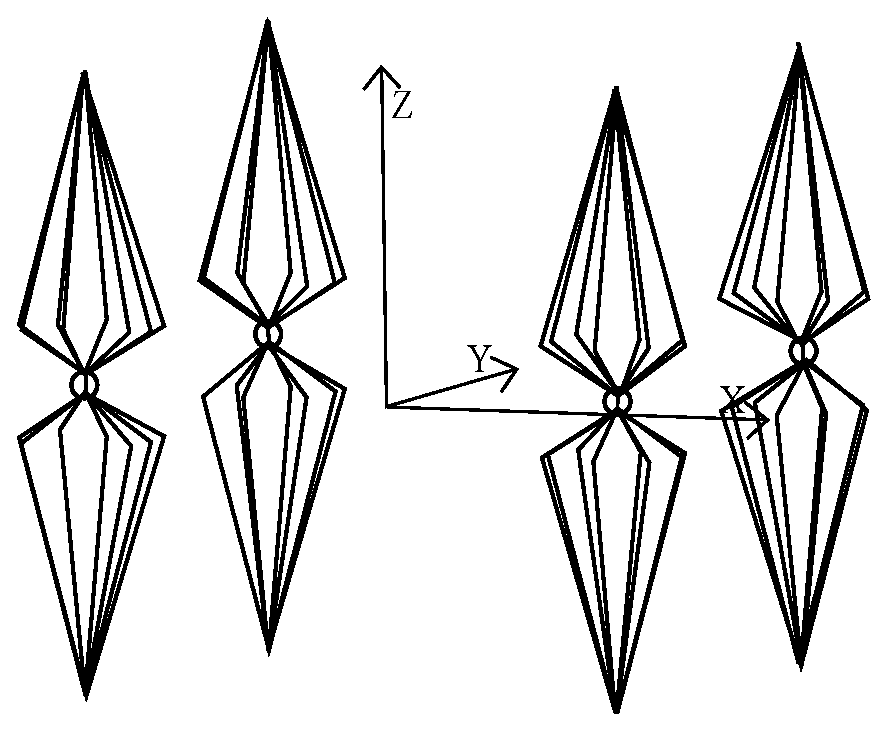
\includegraphics[width=0.6\linewidth]{2x2bvd.eps} \\ б)}
    \end{minipage}
    \begin{minipage}[h]{0.49\linewidth}
        \center{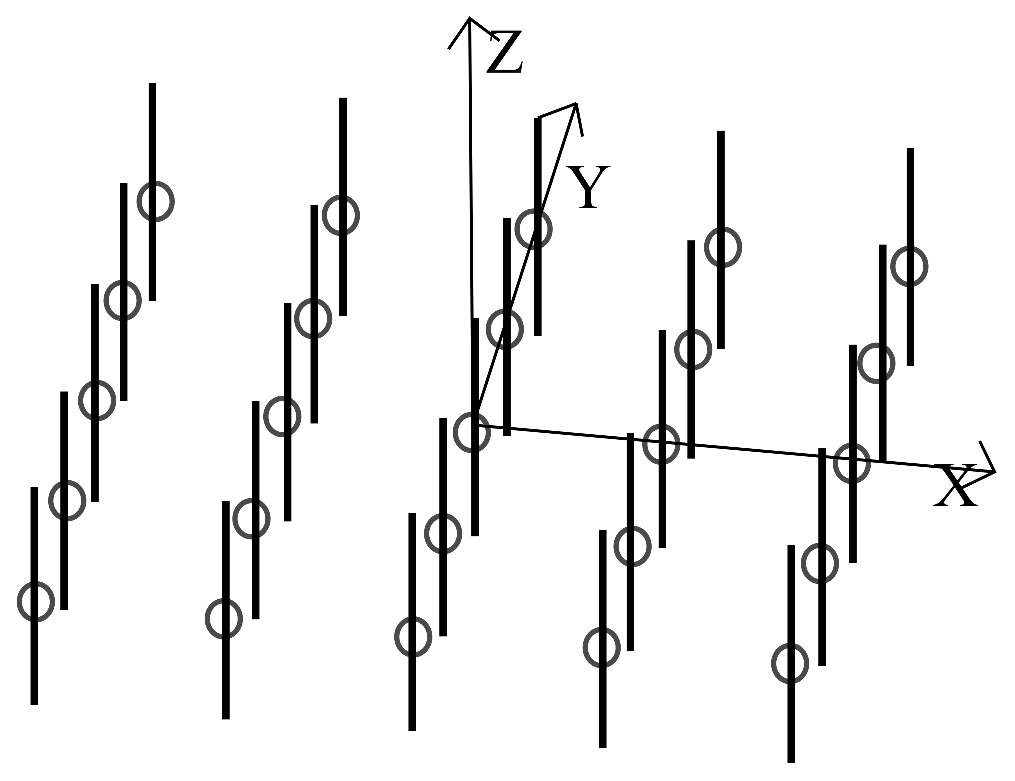
\includegraphics[width=0.6\linewidth]{5x5SVD.eps} \\ в)}
    \end{minipage}
    \hfill
    \begin{minipage}[h]{0.49\linewidth}
        \center{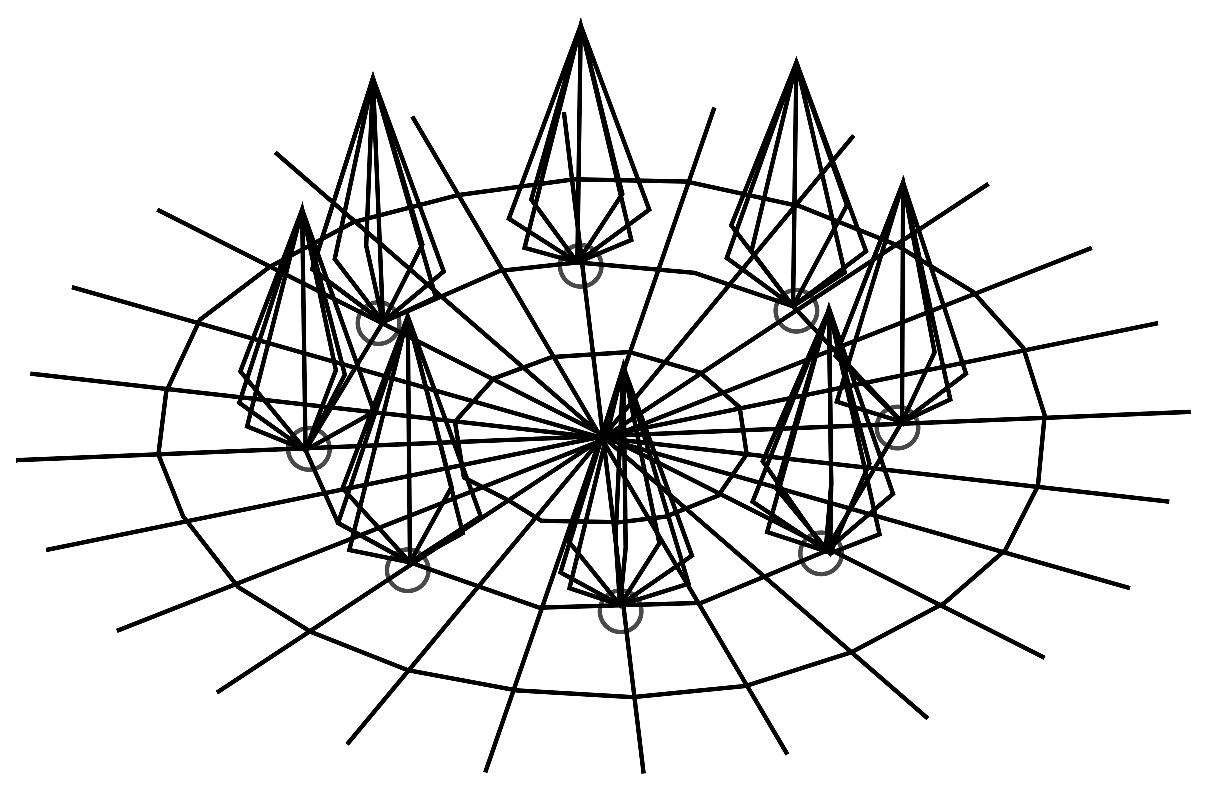
\includegraphics[width=0.9\linewidth]{r8.eps} \\ г)}
    \end{minipage}
    \caption{ФАР различных конфигураций}
    \label{ris:paas}
\end{figure}

Здесь сравниваются результаты работы градиентного метода и решателя BARON в его режиме по умолчанию. Во всех экспериментах, описанных ниже, было установлено ограничение по времени 1000с. Все эксперименты проводились на ЭВМ с процессором Intel i7 (тактовая частота: 2.8ГГц), ОЗУ: 16Гб. В случае остановки градиентного метода (завершение по минимально допустимому приращению целевой функции $10^{-4}$), алгоритм перезапускается заново до истечения запаса времени.

Во время каждой инициализации градиентного метода в главе 1 стартовая точка~$\textbf{x}$ выбирается независимо с равномерным распределением в кубе $[-5000, 5000]^{2N}$. Лучшее из найденных таким образом решений принимается за конечный результат. Параметр штрафа~$r$ в методе градиентной оптимизации установлен равным $10^6$ на всех запусках. Такое значение было определено эмпирически. В таблице~\ref{tab:results} приводятся результаты вычислительного эксперимента. Значения целевой функции ``$\tilde{F}$''в точке, полученной алгоритмом градиентного подъема, приводятся после процедуры масштабирования~(\ref{eq:scale}). Для решателя BARON версии~18.5.8 было выбрано то же самое ограничение сверху на процессорное время, что и для градиентного метода (группа колонок ``BARON''). Во всех таблицах, колонка ``t'' содержит время до получения лучшего найденного решения или до установления глобальной оптимальности. Во всех запусках градиентного метода были получены решения, где активными оказались все ограничения вида $\textbf{x}^{T}\textbf{H}^{(k)}\textbf{x} \leq 1$ и только они.

%Как было показано выше, градиентный метод может предоставить решение, не являющийся локальным оптимумом, если целевая функция слабо изменяется в окрестности текущей точки. Алгоритм дифференциальной эволюции не подвержен такому поведению. Эксперименты показывают, что в целом эволюция популяции соответствует динамике случайного облака точек, движущегося как целое вдоль рельефа оптимизируемой функции, повторяя его характерные особенности. В случае попадания в овраг «облако» принимает форму этого оврага и распределение точек становится таким, что математическое ожидание разности двух случайных векторов оказывается направленным вдоль длинной стороны оврага. Это обеспечивает быстрое движение вдоль узких вытянутых оврагов, тогда как для градиентных методов в аналогичных условиях характерно колебательная динамика «от стенки к стенке». Приведенные эвристические соображения иллюстрируют наиболее важную и привлекательную особенность алгоритма ДЭ — способность динамически моделировать особенности рельефа оптимизируемой функции. Именно этим объясняется замечательная способность алгоритма быстро проходить сложные овраги, обеспечивая эффективность даже в случае сложного рельефа.

Очевидным недостатком градиентного подъема является невозможность выйти из окрестности локального оптимума. Таким образом, данный алгоритм хорошо подходит лишь для работы в режиме множественного запуска или же для уточнения некоторого заданного решения. Такое решение может быть получено алгоритмом дифференциальной эволюции (ДЭ).

Кратко опишем идею алгоритма. В начале происходит генерация популяции. Если нет дополнительной информации, особи популяции генерируются случайным образом с равномерным распределением. Затем, каждая особь подвергается мутации путем присваивания ей признаков другой особи.
Для этого случайным образом выбираются неравные друг другу особи $A$, $B$, $C$. Из них формируется новая особь $C' = C + f(A - B)$, где $f$ -- параметр алгоритма. Из исходной особи и особи $C'$ формируется особь новой популяции. Для этого каждый признак исходной особи с заданной вероятностью $p$ заменяются на соответствующий признак $C'$. Выживает особь с лучшим значением целевой функции.

%В данной работе был предложен вариант реализации алгоритма дифференциальной эволюции, адаптированный для запуска на графическом устройстве.
В данной работе была предложена модификация алгоритма, при которой к особи с лучшим значением целевой функции применяется градиентный алгоритм, если количество итераций алгоритма превышает двухкратного количества итераций, потребовавшегося для получения этого рекорда. По истечении заданного количества итераций к лучшему решению также применяется градиентный подъем. 
%При таком подходе гарантируется сходимость алгоритма к локальному оптимуму, что может не произойти в реализации алгоритма ДЭ.
%Использование алгоритма ДЭ позволило достичь решения с целевой функцией $\tilde{F} = 253$ для задачи СВД'~2x2.

\begin{table}[!h]
\centering
\caption{ Результаты оптимизации, полученные с помощью градиентного подъема, решателя BARON и ДЭ.}
\begin{tabular}{|c|c|c c|c c|c|}
    \hline
    \multirow{2}{*}{\textbf{Тип}} & \multirow{2}{*}{$\sqrt{\frac{N}{\lambda_{\min}}}$} & \multicolumn{2}{c}{\textbf{Град.}} & \multicolumn{2}{|c|}{\textbf{BARON}} & \textbf{ДЭ}\\
    & & \textbf{$\tilde{F}$} & \textbf{t, c} & \textbf{$\tilde{F}$} & \textbf{t, c} & \textbf{$\tilde{F}$} \\
    \hline
    ШВИ 2х2 & 13.6 & 138 & {0.054} & {139} & 0.12 & {139}  \\
    ШВИ 3х3 & 22.5 & 576 & 0.93 & {581} & {0.34} & {581}  \\
    ШВД 2х2 & 21 & 460 & {0.13} & {464} & 0.27 &  {464}  \\
    ШВД 3х3 & 82.2 & 915 & 24.4 & {925} & {0.34} & 924   \\
    СВД 2х2 & 44.7& 357 & 1.9 & {361} & {0.16} & {361}   \\
    СВД 3х3 & 641.9& 1138 & 25.6 & \textbf{1261} & {0.38} & 1163 \\
    СВД 5х5 & $1.1\cdot10^{5}$ & 5318 & 1000 & 6716 & 1000 & \textbf{7132}  \\
    СВД' 2х2 & $2.3\cdot10^{4}$ & 233 & 2.52 & \textbf{253} & {0.25} & 198  \\
    СВД' 3х3 & $6\cdot10^5$& 664 & 71 & \textbf{1153} & {1.48} & 834  \\
    СВД' 5х5 & - & 1382 & 1000 & 33.5 & 217.94 & \textbf{2755}   \\
    Кольц. 8 & 87 & 217 & 8.06 & 218 & {0.23} & 218  \\
    Кольц. 16          & 154 & 727 & 90.9 & 734 & {1.37} & 732  \\
    \hline
\end{tabular}
\label{tab:results}
\end{table}

Из таблицы~\ref{tab:results} видно, что на всех видах решеток, кроме решеток СВД конфигураций~3x3 и~5x5, а также СВД' конфигураций~2x2 и~3x3, разница в значениях целевой функции не превосходит 1\%. Для решеток СВД конфигураций~3x3 и~5x5, а также СВД' конфигураций~2x2 и~3x3 градиентный алгоритм существенно уступает по качеству найденного решения. Кроме решeток ШВИ и ШВД конфигурации~2x2 BARON демонстрирует лучшее время счета. Кроме того, алгоритм ДЭ сравнивался с решателем BARON на пяти задачах из гл.~4 в тех же условиях, что описаны выше. Алгоритм ДЭ на всех примерах нашел допустимые решения, а решатель BARON -- только в четырех примерах. На этих примерах результаты ДЭ отличались не более чем на~1\% по целевой функции от решений BARON.
Cледует отметить, что для обоих алгоритмов время, затраченное на поиск решения, было либо существенно меньше, либо сравнимо со временем, затраченным на построение исходных данных пакетом моделирования NEC, что делает оба подхода равноценными по времени работы с практической точки зрения. При увеличении времени счета BARON до 50000c. для ФАР конфигураций ШВИ~2x2, ШВД~2x2 и ШВИ~3x3 была доказана глобальная оптимальность найденного решателем BARON решения из таблицы~\ref{tab:results}.
%Также показано, что использование комбинированного алгоритма, сочетающего ДЭ и градиентный подъем с адаптацией штрафа, предоставляет не худшие результаты, чем градиентный метод, а в некоторых случаях, даже лучшие, чем BARON. Однако, завершение алгоритма ДЭ требует существенно больше времени.
Из проведенных экспериментов можно сделать вывод о том, что разработанный гибридный вариант ДЭ показывает конкурентоспособные результаты в сравнении с коммерческим решателем BARON в режиме его настроек по умолчанию, при этом преимущество ДЭ наблюдается на задачах с наибольшей размерностью. Решатель ANTIGONE также был опробован в режиме его настроек по умолчанию, но в большинстве тестовых примеров возвращал нулевое решение.

\underline{\textbf{Третья глава}} посвящена исследованию структуры локальных оптимумов с помощью различных алгоритмов оптимизации,
производится анализ наличия групп непрерывных симметрий.

\begin{table}[!h]
\centering
\caption{Структура множества локальных оптимумов.}
\begin{tabular}{|l | l l | c c c | c c c|}
    \hline
    \textbf{ФАР} & \textbf{$M$} & \textbf{$M_{ne}$} & \textbf{$M_{f}$} & \textbf{$\mathcal{B}_{M_f}$} & \textbf{$\mathcal{L}_{M_f}$} & \textbf{$M_{y\approx0}$} & \textbf{$\mathcal{B}_{M_{y\approx0}}$} & \textbf{$\mathcal{L}_{M_{y\approx0}}$}\\
    \hline
    ШВИ 2x2 & 18368 & 4 & 1 & 1 & 1 & 4 & 4 & 4\\
    ШВД 2x2 & 7678  & 4 & 1 & 1 & 1 & 4 & 4 & 4\\
    СВД 2x2  & 523  & 1 & 1 & 1 & 1 & 1 & 1 & 1\\
    СВД 3x3  & 39  & 9 & 2 & 2 & 2 & 5 & 5 & 5\\
    СВД' 2x2  & 396  & 370 & 3 & 3 & 3 & 338 & 1000 & 1213\\
    СВД' 3x3  & 14  & 14 & 3 & 3 & 3 & 1 & 1 & 1\\
    ШВИ 3x3 & 1070  & 3 & 1 & 1 & 1 & 3 & 3 & 3 \\
    ШВД 3x3 & 41  & 4 & 4 & 4 & 4 & 1 & 1 & 1 \\
    Кольц. 8 & 124  & 9 & 2 & 2 & 2 & 9 & 9 & 9\\
    Кольц. 16 & 11  & 6 & 1 & 1 & 1& 6 & 6 & 6\\
    \hline
\end{tabular}
    \label{tab:structure}
\end{table}

\begin{figure}
\centering
    \begin{minipage}[h]{0.8\linewidth}
            \center{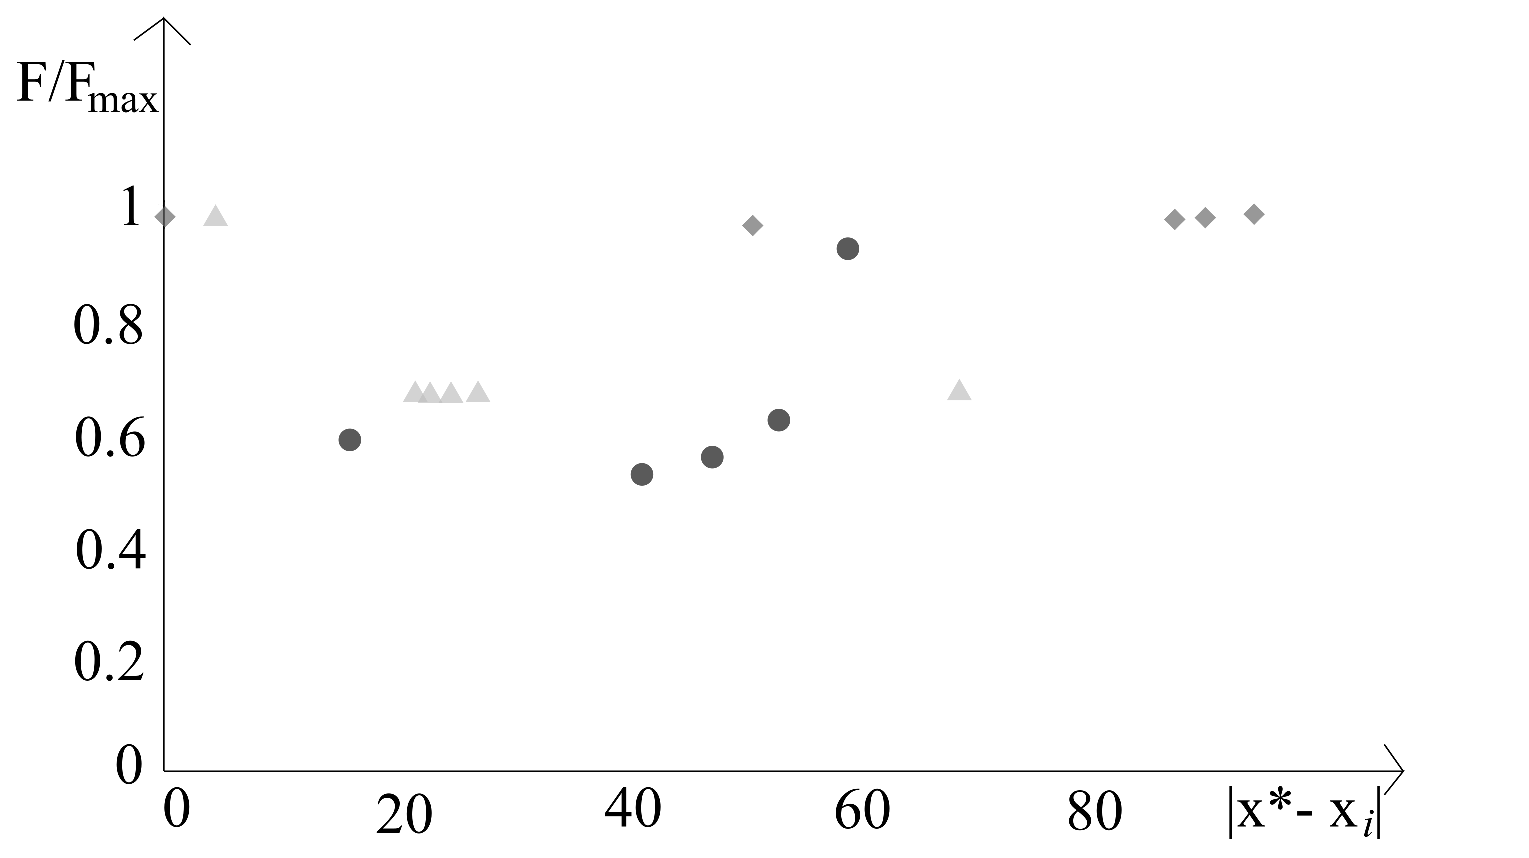
\includegraphics[width=0.9\linewidth]{fit_dist.eps}  \\ а) }
    \end{minipage}
    \begin{minipage}[h]{\linewidth}
            \center{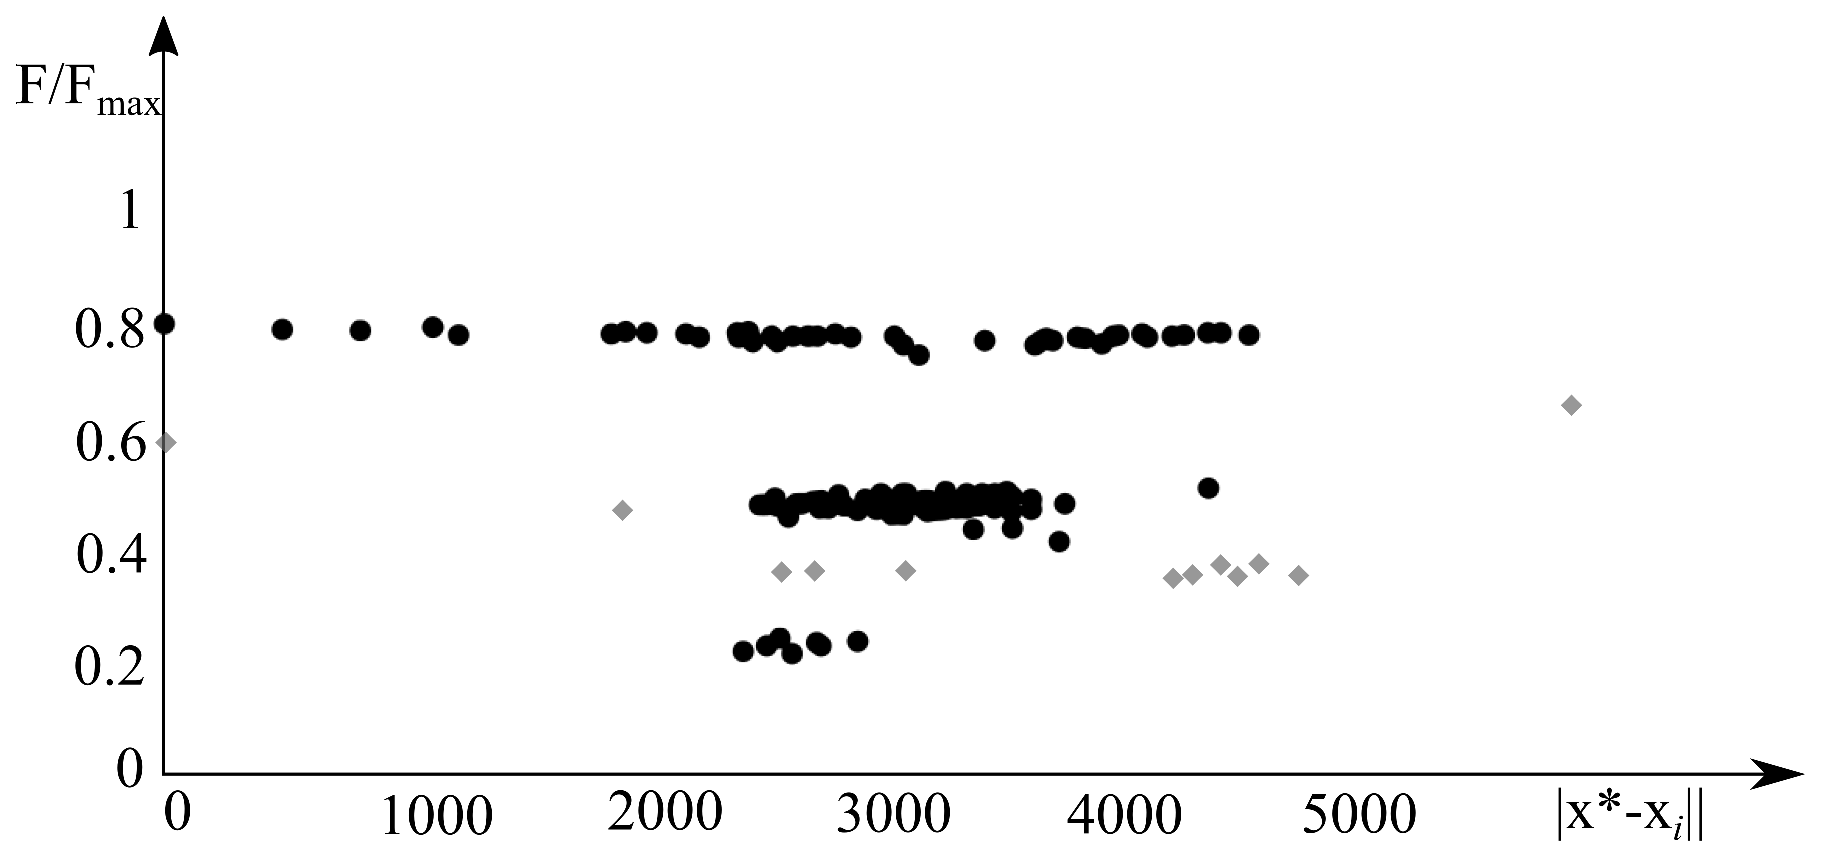
\includegraphics[width=0.9\linewidth]{fit_dist_2x2.eps}  \\ б) }
    \end{minipage}
    \vspace{0.7em}
    \caption{Структура множества найденных решений для задач ШВИ, ШВД, СВД~(а) и~СВД'~(б)}
    \label{ris:fit_dist}
\end{figure}

Для оценки общего числа локальных оптимумов использовался метод переписи Шнабеля. Данный метод имеет применение в экологии и заключается в
выводе статистических оценок численности популяции на основе числа особей, помеченных в результате эксперимента, из популяции с неизменным
составом. В~\mycite{eremeev:confidence}{Еремеев} предлагается адаптация такого метода для оценки числа локальных оптимумов. В таблице~\ref{tab:structure} приводится статистика по числу различных точек остановки (в пределах заданной точности) процедуры мультистарта в течение 1000~с. процессорного времени. Для каждого решения была применена процедура линеаризации задачи и проверки необходимых условий локальной оптимальности. Здесь {$M$} -- число выполненных запусков за отведенное время, $M_{ne}$ -- число групп решений, отличающихся не более чем на 10\% по каждой из координат, {$M_{f}$} -- число групп значений целевой функции у таких неэквивалентных решений (с точностью до 10\%, приведенных в таблице~\ref{tab:results}). {$M_{y\approx0}$} -- число групп решений, для которых были выполнены необходимые условия локальной оптимальности. $\mathcal{B}$ и $\mathcal{L}$ -- оценка нижней границы и оценка максимального правдоподобия числа локальных оптимумов, рассчитанные по методу переписи Шнабеля. Доверительная вероятность для данного метода была выбрана равной 0.95. Оценки для числа решений с различными значениями целевой функции обозначены $\mathcal{B}_{M_f}$ и $\mathcal{L}_{M_f}$. Оценки для числа решений, для которых были выполнены необходимые условия локальной оптимальности, обозначены $\mathcal{B}_{M_{y\approx0}}$ и $\mathcal{L}_{M_{y\approx0}}$.

На рис.~\ref{ris:fit_dist} приведены диаграммы найденных локальных оптимумов, где по оси ординат отложены значения целевой функции, а по оси абсцисс -- расстояние до лучшего известного решения. В случае а) точками обозначены результаты для кольцевых решеток, состоящих из 8 излучателей, ромбами -- для кольцевых решеток, состоящих из 16 излучателей, пятиугольниками - для СВД~3x3. В случае б) точками обозначены результаты для СВД'~2x2, ромбами -- для СВД'~3x3. Диаграмма показывает, что значения, соответствующие одному и тому же значению целевой функции, могут находиться достаточно далеко друг от друга, что позволяет сделать предположение о наличии неучтенных симметрий задачи.

Известно \mycite{yurkov:symmetry}{Юрков}, что любой элемент группы непрерывных симметрий задачи~(\ref{eq:task3}) может быть описан в виде~(\ref{eq:sunexp}).
\begin{equation}
\label{eq:sunexp}
Q=e^{\sum\limits_n a_n G_n} \, .
\end{equation}
где $a_n$ -- вещественные числа, $G_n$ -- генераторы в теоретико-групповом смысле. В качестве генераторов $G_n$ можно выбрать косо-симметричные матрицы, которые содержат над главной диагональю один единичный элемент, симметричный ему противоположный элемент и остальные нули.
Введем матрицу: $ {\textbf{H}}_{\Sigma} = \sum_{i} \textbf{H}_i,$ которая может быть представлена в виде конгруэнтного преобразования диагональной матрицы $D$:
$${\textbf{H}}_{\Sigma} = S^TDS,$$
при некоторой матрице $S$.
Нахождение непрерывных групп симметрий сводится к решению задачи~(\ref{eq:commutat2}).

\begin{equation}
\label{eq:commutat2}
\left\{
\begin{array}{l}
\displaystyle
\tilde{\textbf{H}}_i \left(\sum\limits_na_nG_n\right) =
\left(\sum\limits_na_nG_n\right)\tilde{\textbf{H}}_i \, , \\ \\
\displaystyle
\tilde{\textbf{G}} \left(\sum\limits_na_nG_n\right) = \left(\sum\limits_na_nG_n\right)\tilde{\textbf{G}} \, .
\end{array}
\right.
\end{equation}

\begin{equation}
\tilde{\textbf{G}}=\left(S^{-1}\right)^T \textbf{A} S^{-1} \, , \qquad
\tilde{\textbf{B}_i}=\left(S^{-1}\right)^T \textbf{B}_i S^{-1} \, , \ i=1,\dots,M.
\end{equation}

Вычислительный эксперимент по поиску группы непрерывных симметрий состоит из следующих этапов:
\begin{enumerate}
  \item Предварительная обработка. Возможная неточность данных нивелируется усреднением симметричных компонент матриц (матрицы $\textbf{G}$ и $\textbf{H}$ должны быть симметричны).
  \item %Normalization of matrices $B_i$.
  Преобразование $ {\textbf{H}}_{\Sigma} = \sum_{i} \textbf{H}_i$ к канонической форме используя метод Лагранжа для вычисления матриц~$S$ и $S^{-1} $.
  \item Применение метода Гаусса к системе линейных уравнений~(\ref{eq:commutat2}) для вычисления генераторов~$\hat{G}_n$.
\end{enumerate}

%\subsection{Optimization of the Excitation of Antenna Arrays}

Описанная процедура нахождения непрерывных групп симметрий применяется к примерам, описанным в главе 1. Для всех рассмотренных задач было выявлено только наличие фазовой симметрии. Предположительно, множественность решений объясняется наличием дискретных симметрий. Выявление дискретных симметрий является объектом дальнейших исследований.

\underline{\textbf{Четвертая глава}} посвящена исследованию возможности оптимизации возбуждения ФАР в различных условиях.

На практике использование высокосимметричных ФАР вызывает особый интерес, так как позволяет выполнить расчеты для одного направления и затем легко адаптировать их для других симметричных направлений. Другой особенностью, влияющей на результаты моделирования является наличие потерь в земле \mycite{yurkov:groundloss}{Юрков}. Чтобы ослабить этот эффект, антенные системы с противовесами подняты над землей на 2 м.

В данной главе мы изучаем, как изменяется общий коэффициент усиления кольцевой ФАР с ростом радиочастоты и плотности системы противовесов. Общий коэффициент усиления является суммой частичных коэффициентов усиления в  двух ортогональных поляризациях. Плотность системы противовесов определяется числом продольных и поперечных проводов, относящихся к одному и тому же излучателю. Частота изменяется от 5 до 30 МГц. Вычисления производились на решетках ШВИ, состоящих из 8 излучателей. Для расчета матрицы сопротивлений и матрицы излучений использовался пакет моделирования антенных систем NEC2.

Для проведения вычислительного эксперимента использовался решатель BARON в пакете GAMS. Результаты оптимизации направленности решетки сравниваются с коэффициентом усиления одиночного излучателя, установленного в центре такой же системы противовесов. Плотность системы противовесов обозначается в формате $long:trans$, где $long$ -- число продольных проводов, относящихся к одному излучателю, а $trans$ -- поперечных. Высота каждого ШВИ -- 15м. В качестве направления оптимизации выбирается $70^{\circ}$ полярного угла и $45^{\circ}$ азимутального угла в сферических координатах.

\begin{figure}
\center{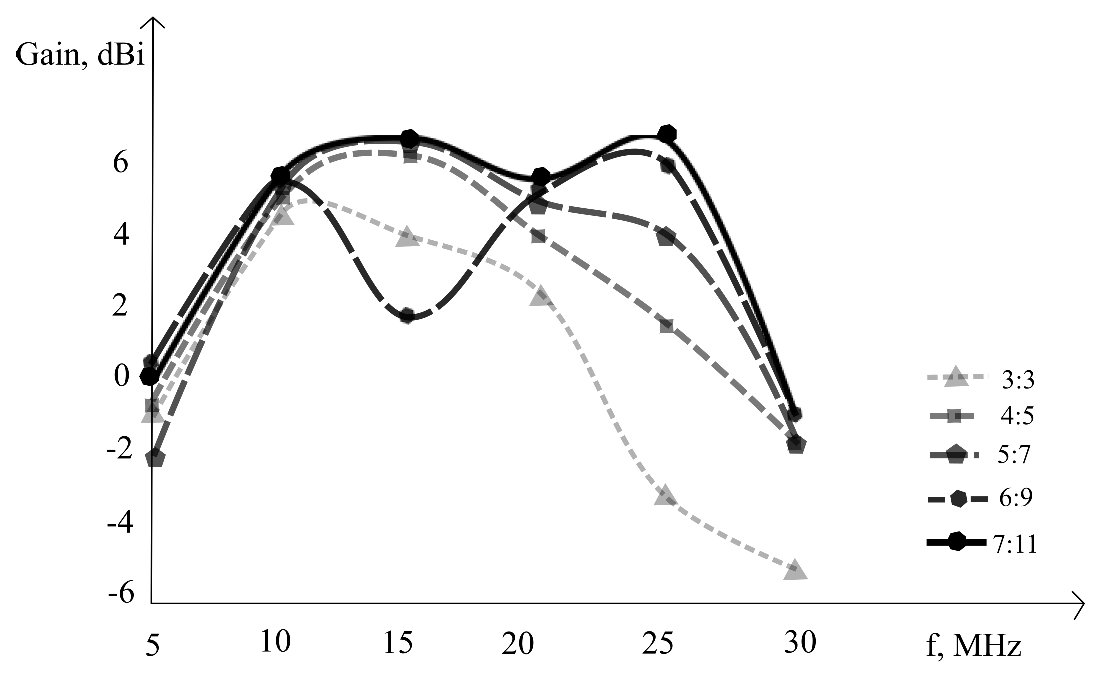
\includegraphics[width=0.8\linewidth]{ring_f__paa_gains.eps}}
\caption{Зависимость от частоты общего коэффициента усиления ФАР при оптимизации в направлении 70:45}
\label{ris:paa_gains}
\end{figure}

На рис.~\ref{ris:paa_gains} показано, как изменяется коэффициент усиления с ростом радиочастоты. Мы можем наблюдать, что при значениях частоты 5 и 30 МГц решетка оптимизируется малоэффективно. Также можно увидеть, что, в основном, увеличение плотности системы противовесов приводит к росту коэффициента усиления.

\begin{figure}
\center{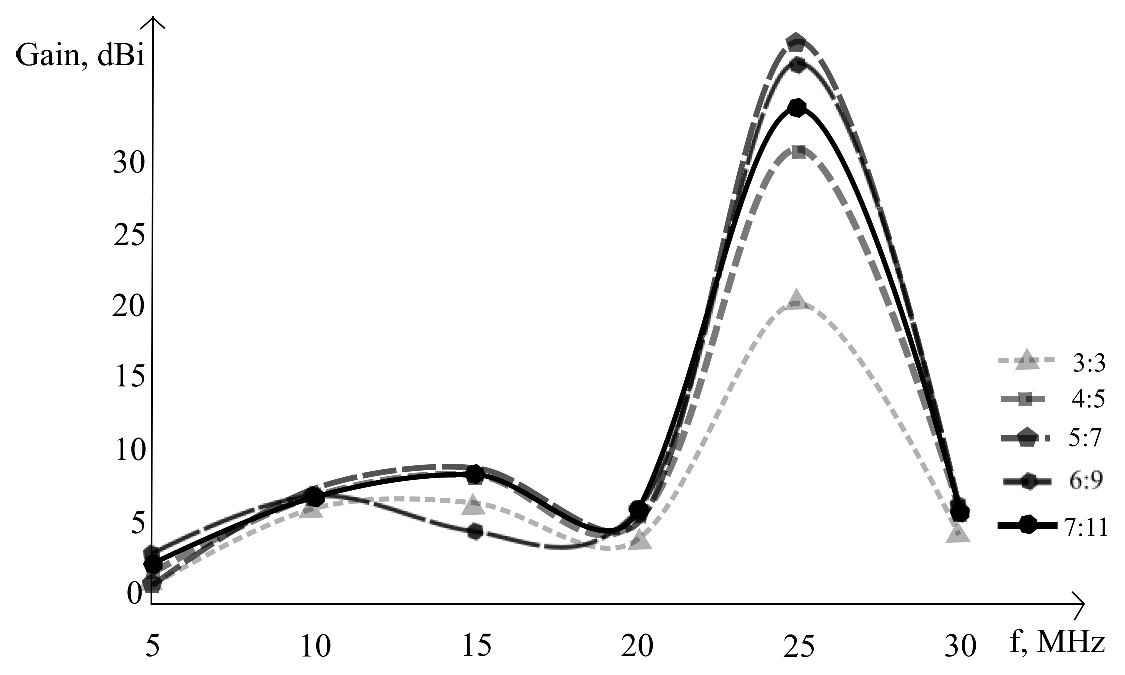
\includegraphics[width=0.8\linewidth]{ring_f_gains.eps}}
\caption{Сравнение коэффициентов усиления ФАР и одиночного излучателя}
\label{ris:all_gains}
\end{figure}

На рис.~\ref{ris:all_gains} показано, как изменяется соотношение коэффициентов усиления ФАР и одиночного излучателя с ростом частоты. Заметным результатом здесь является то, что на частоте 25МГц усиление ФАР существенно больше усиления одиночного излучателя. Объяснение этого эфффекта будет приведено далее при сравнении диаграмм направленности.

\begin{figure}
\begin{minipage}[h]{0.49\linewidth}
\center{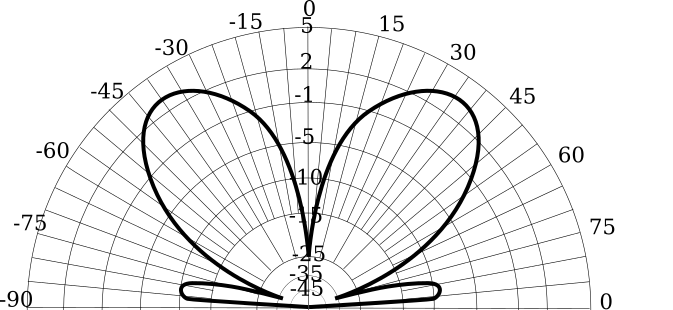
\includegraphics[width=1\linewidth]{r8_1_25_5x7.png} \\ а)}
\end{minipage}
\hfill
\begin{minipage}[h]{0.49\linewidth}
\center{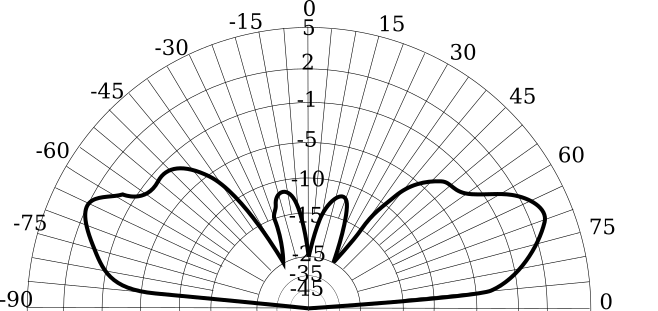
\includegraphics[width=1\linewidth]{r8_25_5x7.png} \\ б)}
\end{minipage}
\caption{Вертикальный план диаграммы направленности одиночного излучателя (а) и ФАР 5:7 (б) при 25МГц}
\label{ris:f25mhs}
\end{figure}

На частоте 25МГц (см~Рис.~\ref{ris:f25mhs}), где усиление ФАР существенно больше усиления одиночного излучателя. Одиночный излучатель довольно мало излучает в направлении оптимизации, тогда как ФАР имеет максимум излучения в этом направлении. Было предположено, что такой эффект был получен вследствие учета взаимного влияния. Согласно~(\ref{eq:A}), если пренебречь взаимным влиянием излучателей, плотность мощности $F$ будет максимальна, когда поля будут синфазны. Для проверки гипотезы о необходимости учета взаимного влияния произведено сравнение диаграмм направленности решеток разных конфигураций после математической оптимизации их направленности в заданном направлении согласно модели~(\ref{eq:task3}) с соответствующими диаграммами одиночного излучателя и со случаем фазирования решетки без учета взаимного влияния (далее – простое фазирование).

Высота каждого ШВИ равна 15~м. Длина плеча симметричных излучателей также равна 15~м. Направление оптимизации по умолчанию было установлено на $70^{\circ}$ полярного угла и $45^{\circ}$ азимутального угла в сферических координатах. Для некоторых экспериментов было проведено дополнительное исследование при $85^{\circ}$ полярного угла.


Для ШВД производилось исследование диаграмм направленности при варьировании расстояния центров излучателей до центра решетки от~5 до 50~м. В большинстве случаев, использование решения задачи математического программирования не давало существенного преимущества перед простым фазированием. Тем не менее, при расстоянии между центром излучателя и центром решетки равным 20~м. это различие составило около 4~дБ~(см.~Рис.~\ref{pic:r_bvd_result}).

\begin{figure}
\begin{minipage}[h]{0.49\linewidth}
\center{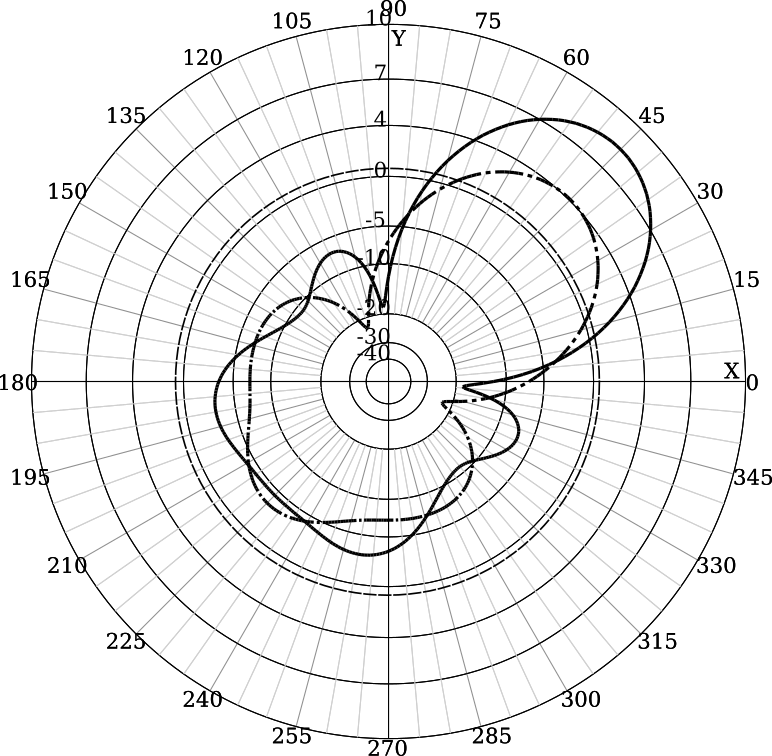
\includegraphics[width=1\linewidth]{r_bvd_20_results_h.png} \\ а)}
\end{minipage}
\hfill
\begin{minipage}[h]{0.49\linewidth}
\center{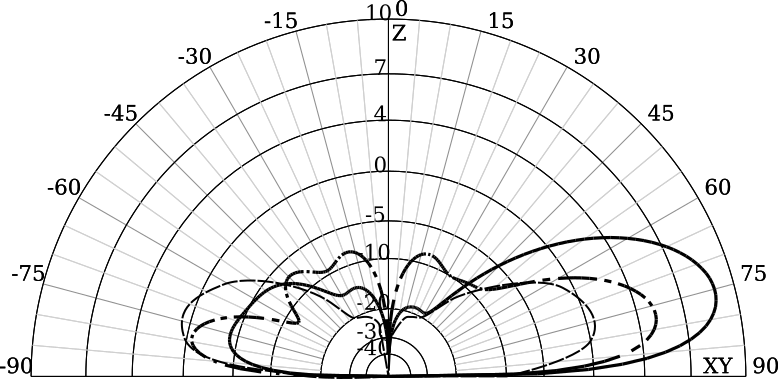
\includegraphics[width=1\linewidth]{r_bvd_20_results_v.png} \\ б)}
\end{minipage}
\caption{Горизонтальный (а) и вертикальный (б) план диаграммы направленности ШВД при расстоянии от центра излучателя до центра решетки 20 м. Пунктирной линией обозначено усиление одиночного излучателя, штрихпунктирной – простое фазирование, сплошной – решение задачи мат. программирования.}
\label{pic:r_bvd_result}
\end{figure}

Аналогичные результаты были получены и для решеток~СВД. При оптимизации в направлении полярного угла равном $70^{\circ}$ при варьировании расстояния от центра излучателя до центра решетки от~35 до 37~м. различие между коэффициентом усиления решения задачи математического программирования и усилением простого фазирования также достигало 4~дБ.  При оптимизации в направлении полярного угла равном $85^{\circ}$ при варьировании расстояния от центра излучателя до центра решетки от 25 до 29~м. эта разница достигала 5~дБ.

\FloatBarrier
\pdfbookmark{Заключение}{conclusion}                                  % Закладка pdf
В \underline{\textbf{заключении}} приведены основные результаты работы, которые заключаются в следующем:
%% Согласно ГОСТ Р 7.0.11-2011:
%% 5.3.3 В заключении диссертации излагают итоги выполненного исследования, рекомендации, перспективы дальнейшей разработки темы.
%% 9.2.3 В заключении автореферата диссертации излагают итоги данного исследования, рекомендации и перспективы дальнейшей разработки темы.
\begin{enumerate}
  \item В текущей работе была рассмотрена постановка задачи оптимизации направленности излучения антенной системы, представленной в виде регулярной решетки излучателей. Для данной задачи была разработана модель квадратичного программирования в вещественных числах. Произведено сравнение результатов разработанных алгоритмов в вычислительном эксперименте.
  \item Проведены вычислительные эксперименты, выявляющие наличие непрерывных групп симметрий допустимых решений. Для всех рассмотренных задач выявлено наличие только фазовой симметрии.
  \item В рамках данного исследования было выявлено наличие ситуаций, в которых коэффициент усиления, соответствующий решению задачи математического программирования, имеет существенное преимущество перед коэффициентом усиления простого фазирования. Выявлено, что, при оптимизации направленности ФАР КВ диапазона целесообразны расчеты с учетом взаимного влияния излучателей.
  \item Для генерации тестовых примеров, автоматизации вычислительных экспериментов и визуализации их результатов были разработаны интерпретатор <<Expi>> и его графическая оболочка <<ExpiIDE>>.
\end{enumerate}


В \underline{\textbf{приложениях}} приводятся формальные описания использованных алгоритмов, а также дается описание разработанного программного комплекса для решения произвольных задач оптимизации ФАР КВ диапазона.
%Для проведения вычислительных экспериментов был разработан интерпретатор <<Expi>> и его графическая оболочка <<ExpiIDE>>.

%Формат языка <<Expi>> позволяет в декларативной форме объявлять правила построения моделей и задавать параметры запуска экспериментов.
%В языке <<Expi>> предоставлены возможности моделировать конфигурации проводников в зависимости от динамических параметров, объединять их в группы и применять к ним геометрические преобразования. Также имеется возможность экспорта определенных конфигураций в формат NEC. Отдельно следует отметить возможность языка выполнять серии вычислительных экспериментов. В <<Expi>> уже встроен интерфейс для работы с пакетом GAMS, а также имеется возможность интеграции любого пользовательского пакета.

%Графическая оболочка <<ExpiIDE>> представляет собой файловый инспектор с возможностью редактировать и запускать файлы экспериментов exp, просматривать и экспортировать диаграммы направленности и геометрию антенных систем.

\pdfbookmark{Литература}{bibliography}

\ifdefmacro{\microtypesetup}{\microtypesetup{protrusion=false}}{} % не рекомендуется применять пакет микротипографики к автоматически генерируемому списку литературы
\urlstyle{rm}                               % ссылки URL обычным шрифтом
\ifnumequal{\value{bibliosel}}{0}{% Встроенная реализация с загрузкой файла через движок bibtex8
    \renewcommand{\bibname}{\large \bibtitleauthor}
    \nocite{*}
    \insertbiblioauthor           % Подключаем Bib-базы
    %\insertbiblioexternal   % !!! bibtex не умеет работать с несколькими библиографиями !!!
}{% Реализация пакетом biblatex через движок biber
    % Цитирования.
    %  * Порядок перечисления определяет порядок в библиографии (только внутри подраздела, если `\insertbiblioauthorgrouped`).
    %  * Если не соблюдать порядок "как для \printbibliography", нумерация в `\insertbiblioauthor` будет кривой.
    %  * Если цитировать каждый источник отдельной командой --- найти некоторые ошибки будет проще.
    %
    %%
    \nocite{tyu:daor}%
    \nocite{tyu:jphys}%
    \nocite{tyu:motor}%
    \nocite{tyu22:ring}%
    \nocite{tyu:opta}%
    \nocite{tyu:reis}%
    \nocite{tyu:fmh}%
    \nocite{tyu:de_sym}%

    %

    \ifnumgreater{\value{usefootcite}}{0}{
        \begin{refcontext}[labelprefix={}]
            \ifnum \value{bibgrouped}>0
                \insertbiblioauthorgrouped    % Вывод всех работ автора, сгруппированных по источникам
            \else
                \insertbiblioauthor      % Вывод всех работ автора
            \fi
        \end{refcontext}
    }{
        \ifnum \totvalue{citeexternal}>0
            \begin{refcontext}[labelprefix=A]
                \ifnum \value{bibgrouped}>0
                    \insertbiblioauthorgrouped    % Вывод всех работ автора, сгруппированных по источникам
                \else
                    \insertbiblioauthor      % Вывод всех работ автора
                \fi
            \end{refcontext}
        \else
            \ifnum \value{bibgrouped}>0
                \insertbiblioauthorgrouped    % Вывод всех работ автора, сгруппированных по источникам
            \else
                \insertbiblioauthor      % Вывод всех работ автора
            \fi
        \fi
        %  \insertbiblioauthorimportant  % Вывод наиболее значимых работ автора (определяется в файле characteristic во второй section)
        \begin{refcontext}[labelprefix={}]
            \insertbiblioexternal            % Вывод списка литературы, на которую ссылались в тексте автореферата
        \end{refcontext}
        % Невидимый библиографический список для подсчёта количества внешних публикаций
        % Используется, чтобы убрать приставку "А" у работ автора, если в автореферате нет
        % цитирований внешних источников.
        \printbibliography[heading=nobibheading, section=0, env=countexternal, keyword=biblioexternal, resetnumbers=true]%
    }
}



\ifdefmacro{\microtypesetup}{\microtypesetup{protrusion=true}}{}
\urlstyle{tt}                               % возвращаем установки шрифта ссылок URL

      % Содержание автореферата

%%% Выходные сведения типографии
\newpage\thispagestyle{empty}

\vspace*{0pt plus1fill}

\small
\begin{center}
    \textit{\thesisAuthor}
    \par\medskip

    \thesisTitle
    \par\medskip

    Автореф. дис. на соискание ученой степени \thesisDegreeShort
    \par\bigskip

    %Подписано в печать \blank[\widthof{999}].\blank[\widthof{999}].\blank[\widthof{99999}].
    %Заказ № \blank[\widthof{999999999999}]

    %Формат 60\(\times\)90/16. Усл. печ. л. 1. Тираж 100 экз.
    %Это не совсем формат А5, но наиболее близкий, подробнее: http://ru.wikipedia.org/w/index.php?oldid=78976454

    %Типография \blank[0.5\linewidth]
\end{center}
\cleardoublepage

\end{document}
